%%%%%  Decoder %%%%%
\subsection{Reconstruction Quality Evaluation}

Our implementation of the Universal Style Transfer is adapted to use two different sets of encoder-decoder models: the models we trained according to section \ref{subsec:Models} (our), and the models offered to download by Li et al in their GitHub (reference). This means that we can test \textbf{our implementation} of the UST algorithm with both sets of models. In this section we want to evaluate our models in comparison to the references in terms of image reconstruction, in order to asses the quality of our models training.

\subsubsection{Quantative Reconstruction Loss}
As section \ref{subsec:Models} explains, the models are trained for image reconstruction. Passing an input image through the encoder-decoder models will output a reconstructed image, featuring some distortion. A better trained model will output images which feature smaller distortion. In order to quantify the reconstruction distortion induced by our trained models, in comparison to that of the reference models, we encode and then decode 1k content images from the COCO dataset with each of the 5 encoder-decoder pairs, and measure the pixel MSE and feature MSE. The pixel MSE measures the pixel mean square error between the reconstructed image, $\hat{x}$, and the original one, $x$, i.e. $MSE(x - \hat{x})$. The feature MSE measures the error between the deep features of the reconstructed image and the original one. It is measured by encoding $x$ and $\hat{x}$ and calculating $MSE(E(x)-E(\hat{x}))$. Table ~\ref{Tab:loss} displays the pixel loss (feature loss) per model, which is defined to be the average pixel MSE (feature MSE) over all 1k images.

% ecoder-decoder table %

\begin{center}
	\captionof{table}{Pixel and Feature Loss Per Model\label{Tab:loss}}
	\centering
	\begin{tabular}{ |>{\centering}p{2.5cm}||>{\centering}p{2.5cm}|>{\centering}p{2.5cm}|>{\centering}p{2.5cm}|>{\centering}p{2.5cm}| }
		\hline
		\multicolumn{5}{|c|}{\hspace{1.4cm} Pixel loss[$1\mathrm{e}{-4}$] \hspace{3cm}$\mid$ \hspace{1cm} Feature loss[$1\mathrm{e}{-2}$]} \\
		\hline
		architecture &Reference &Our &Reference &Our \tabularnewline
		\hline
		1 &$8.246$  &$802$   &$2.161$ &$0.7$\tabularnewline
		\hline
		2 &$2.374$  &$810$   &$1.257$ &$15.30$\tabularnewline
		\hline
		3 &$7.994$  &$884$   &$16.38$ &$86.60$\tabularnewline
		\hline
		4 &$0.281$  &$830$   &$25.09$ &$223.6$\tabularnewline
		\hline
		5 &$107.4$  &$818.6$   &$108.0$ &40.52\tabularnewline
		\hline
	\end{tabular}\\
\end{center}

\textcolor{red}{TODO: complete when 5th row is complete...} From table ~\ref{Tab:loss} it is visible that in terms of pixel loss, the reconstruction done by the reference models is at least two orders of magnitude better than of our models. It is also visible that the  pixel loss generally increases as the architecture gets deeper. In addition, we measure quantitatively (see table ~\ref{Tab:loss}) our reconstruction distortion loss by two measures: pixel loss and feature loss as depicted in equation \ref{eq:loss} and elaborated in \cite{bib22, bib17}.\newline\\

%%%%%%%%%%%%%%%%%%%%%%%%%%%%%%%%%%%%%%%%%%
%%% reconstruction comparison %%%
%%%%%%%%%%%%%%%%%%%%%%%%%%%%%%%%%%%%%%%%%%
\subsubsection{Qualitative Reconstruction Loss}
To demonstrate the image reconstruction performance of our trained models, we choose 5 different images and feed them as input to both our encoder-decoder architectures, and the references. The results, as presented in figure ~\ref{fig:reconstruction}, visualize the image reconstruction quality of our models in comparison to that of the references. Column (a) consists of the original images, (b) presents the reconstruction results for encoder-decoder architecture \#1, columns (c)-(f) present the same for architectures 2-5 as depicted in \ref{subsec:Models}, and column (g) presents the reconstruction result done by the reference encoder-decoder architecture \#5. 

%%%%%%%%%%%%%%%%%%%%%%%%%%%%%% Reconstrucion images %%%%%%%%%%%%%%%%%%%%%%%%%%%%%%%%%%
\begin{figure}[H]
	% first line
	\centering
	\begin{subfigure}[b]{0.13\linewidth}
		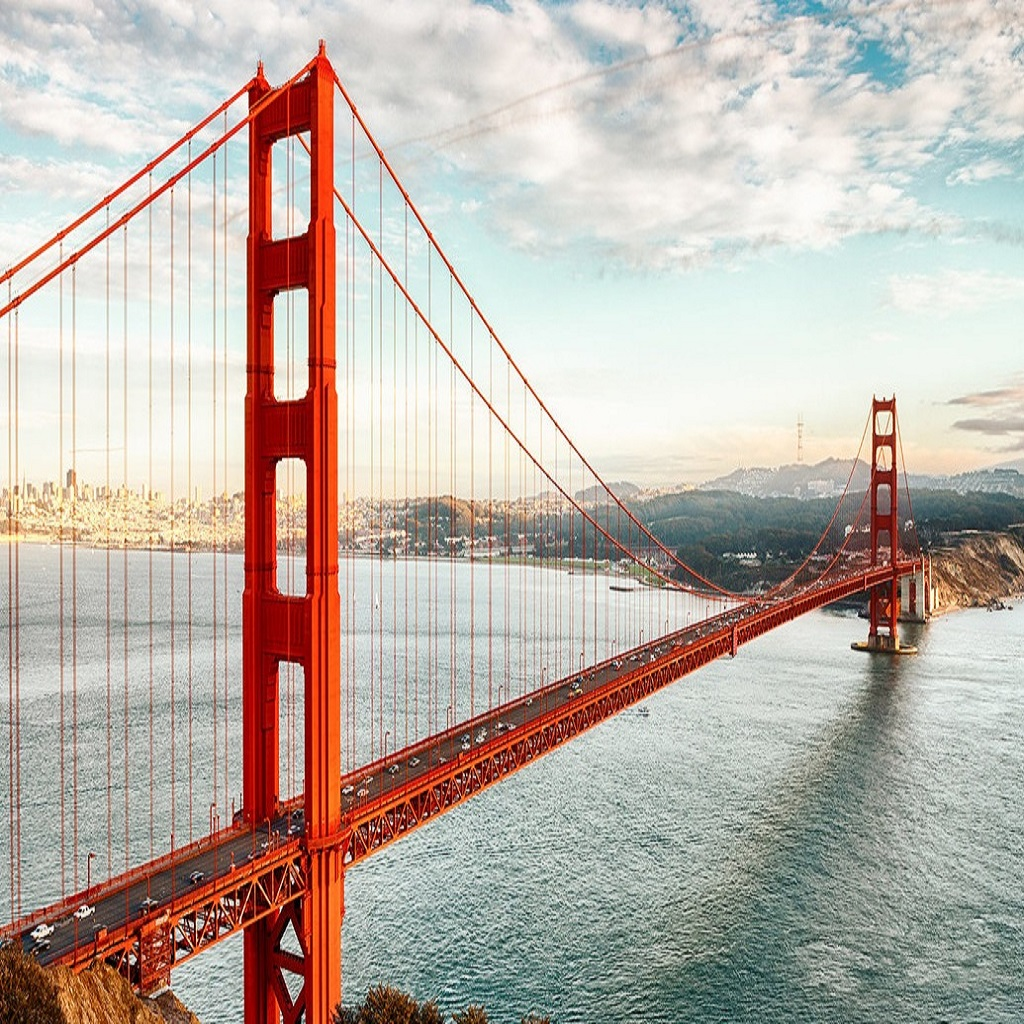
\includegraphics[width=\linewidth]{bridge_sq.jpg} % original num.1	
	\end{subfigure}
	\begin{subfigure}[b]{0.13\linewidth}
		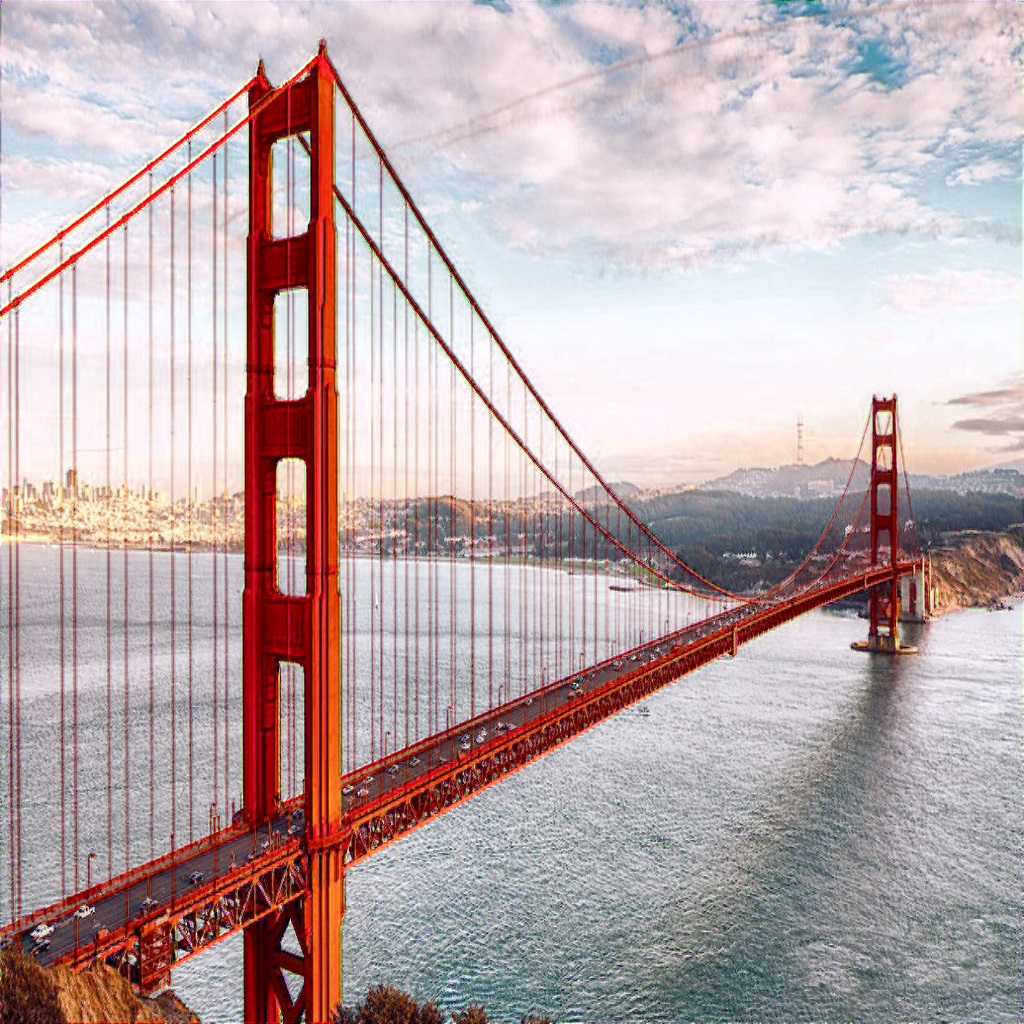
\includegraphics[width=\linewidth]{reconst_exper/dec_bridge_my_1_test.jpg} % our reconstruction arc1 num.1	
	\end{subfigure}
	\begin{subfigure}[b]{0.13\linewidth}
		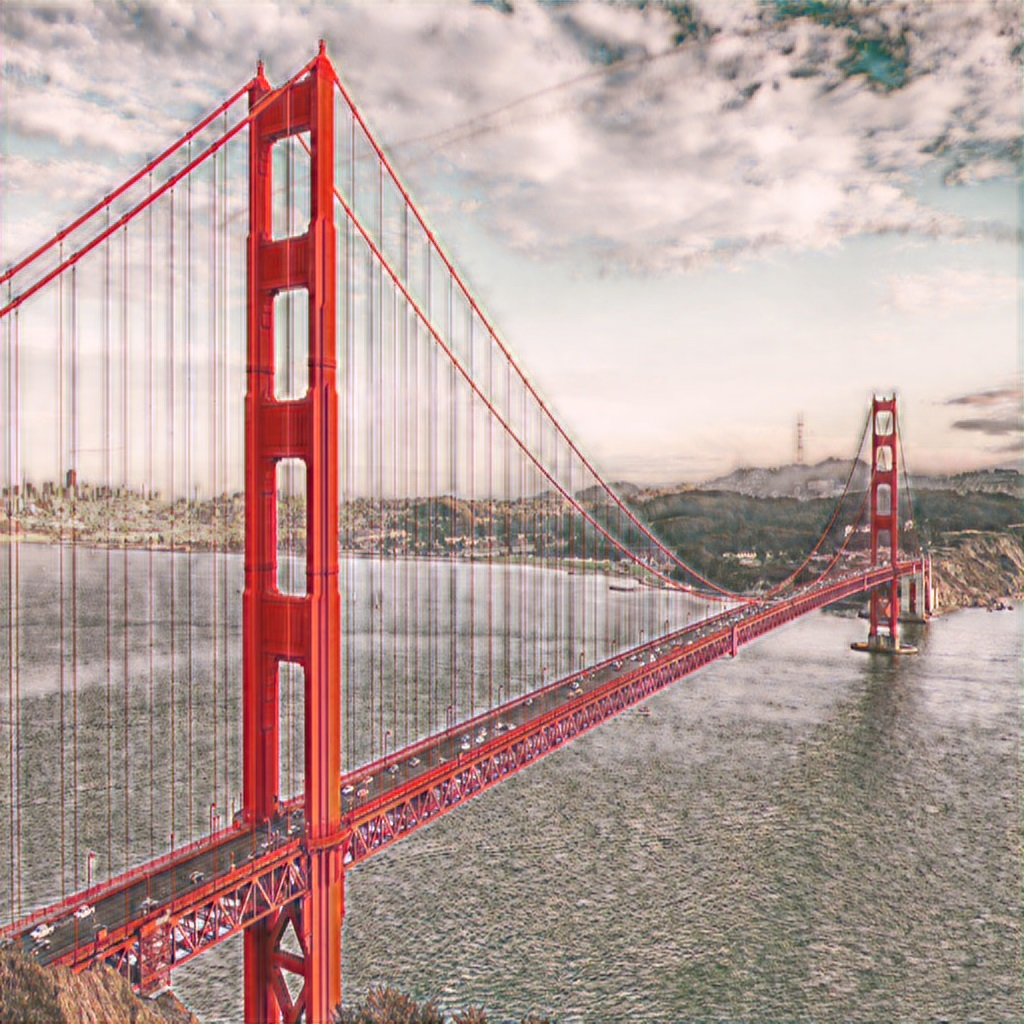
\includegraphics[width=\linewidth]{reconst_exper/dec_bridge_my_2_test.jpg} % our reconstruction arc2 num.1	
	\end{subfigure}
	\begin{subfigure}[b]{0.13\linewidth}
		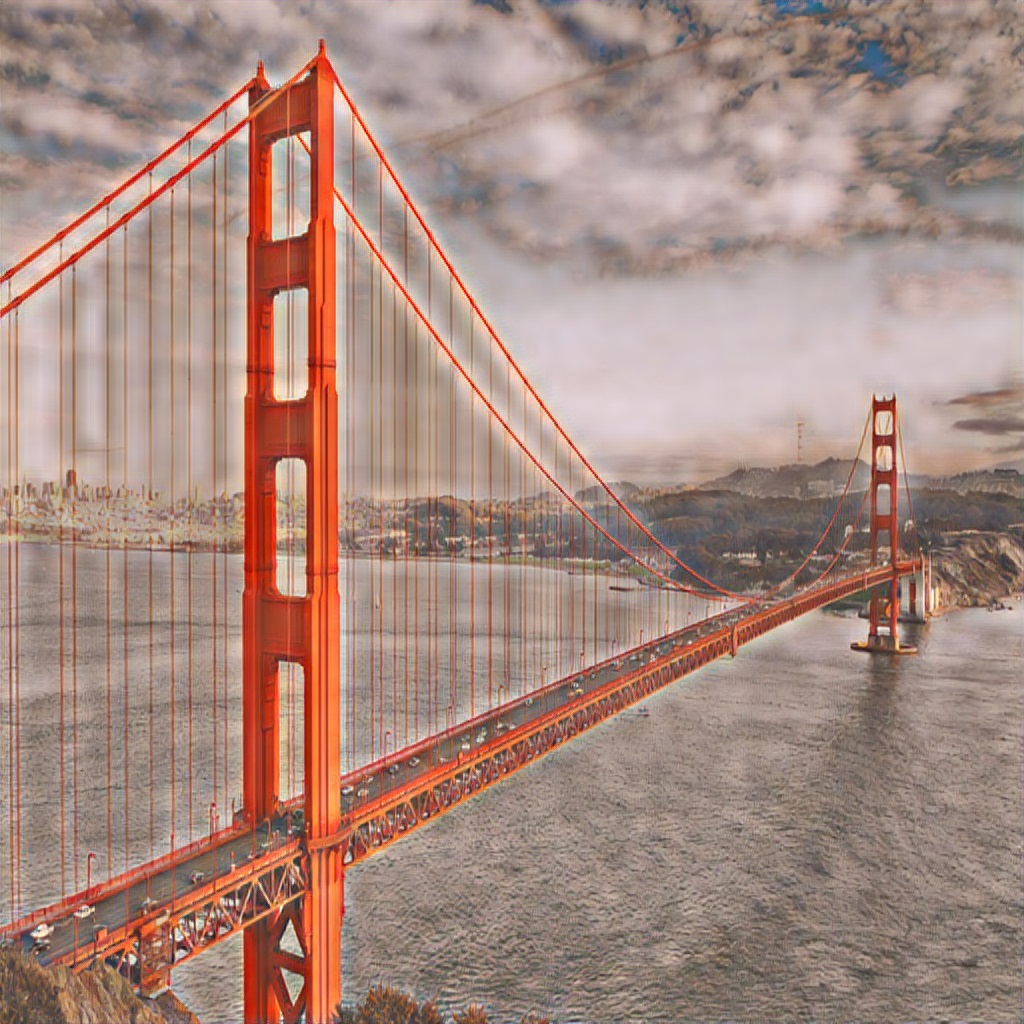
\includegraphics[width=\linewidth]{reconst_exper/dec_bridge_my_3_test.jpg} % our reconstruction arc3 num.1	
	\end{subfigure}
	\begin{subfigure}[b]{0.13\linewidth}
		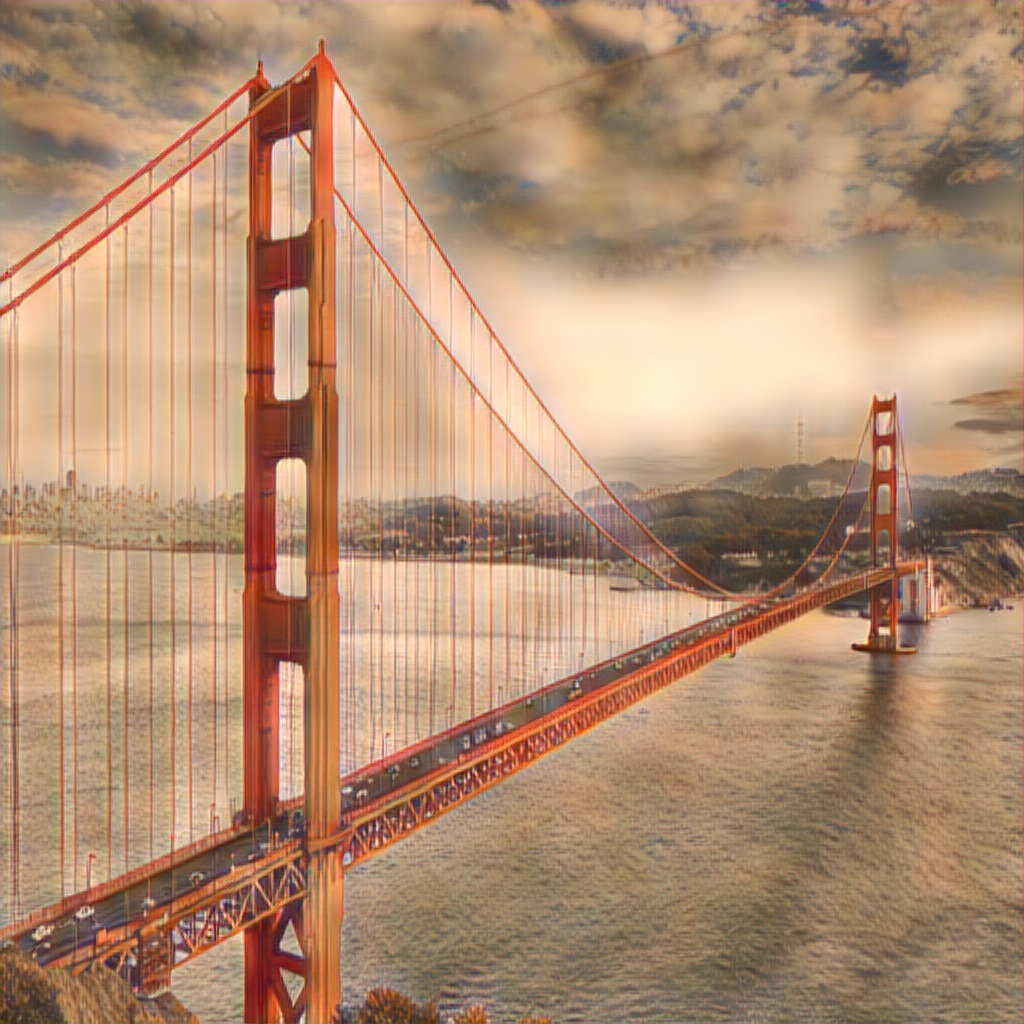
\includegraphics[width=\linewidth]{reconst_exper/dec_bridge_my_4_test.jpg} % our reconstruction arc4 num.1	
	\end{subfigure}
	\begin{subfigure}[b]{0.13\linewidth}
		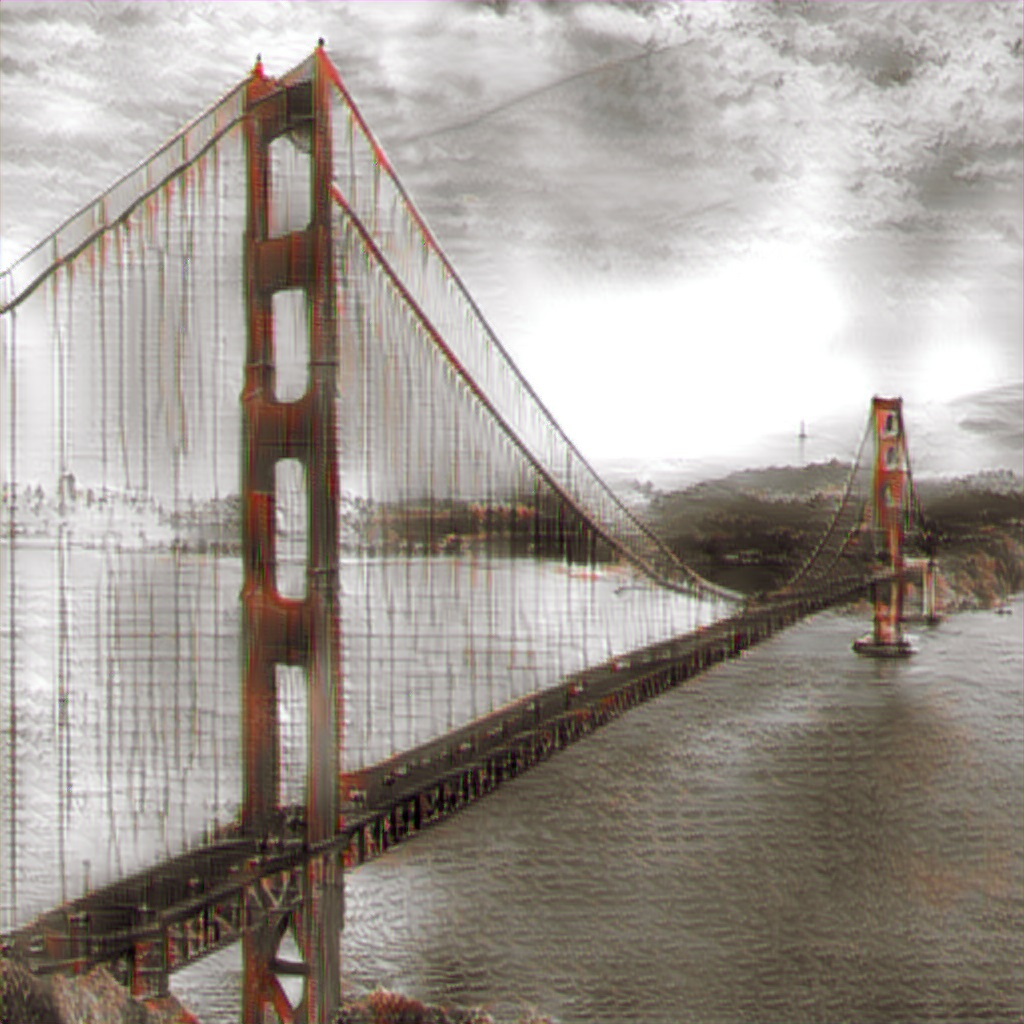
\includegraphics[width=\linewidth]{reconst_exper/dec_bridge_my_5_test.jpg} % our reconstruction arc5 num.1	
	\end{subfigure}
	\begin{subfigure}[b]{0.13\linewidth}
		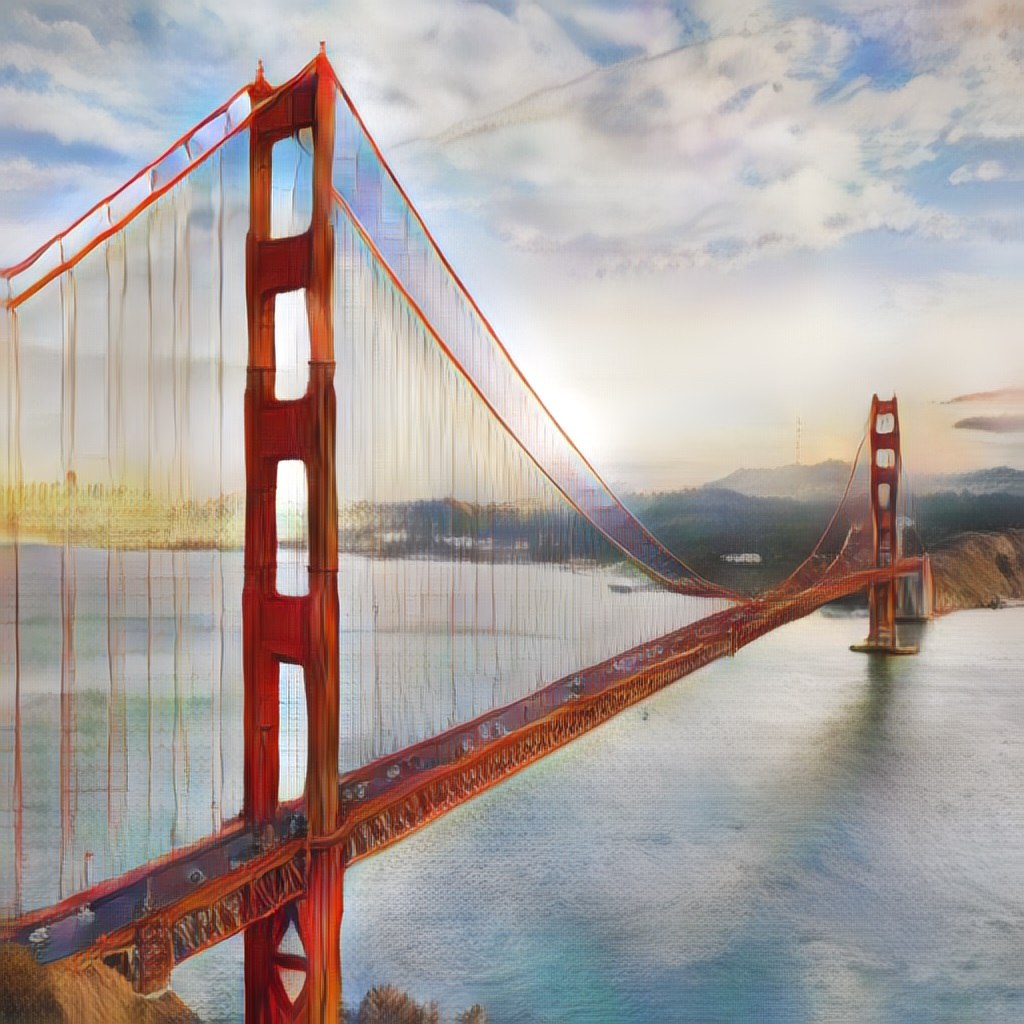
\includegraphics[width=\linewidth]{reconst_exper/dec_bridge_ref_5_test.jpg} % their reconstruction arc5 num.1	
	\end{subfigure}
	% second line
	\centering
	\begin{subfigure}[b]{0.13\linewidth}
		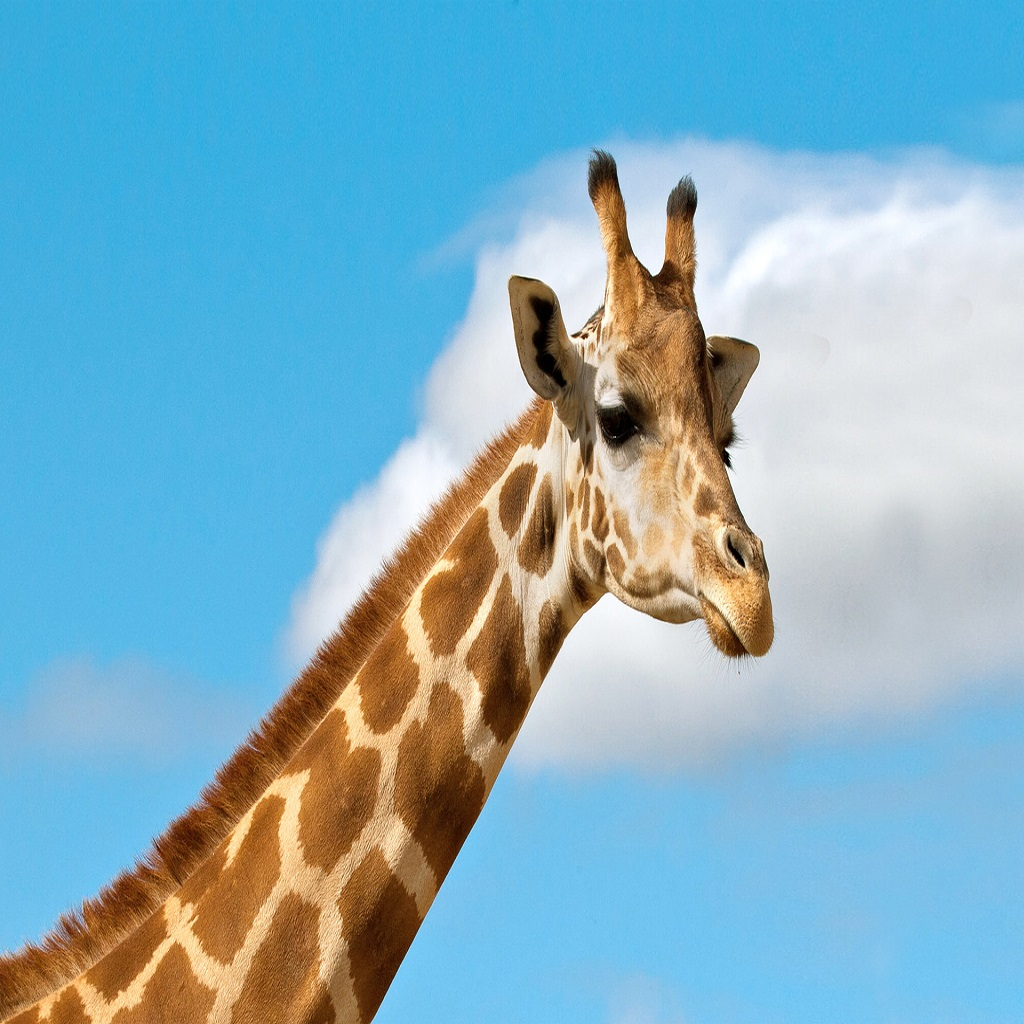
\includegraphics[width=\linewidth]{giraffe_sq.jpg} % original num.1	
	\end{subfigure}
	\begin{subfigure}[b]{0.13\linewidth}
		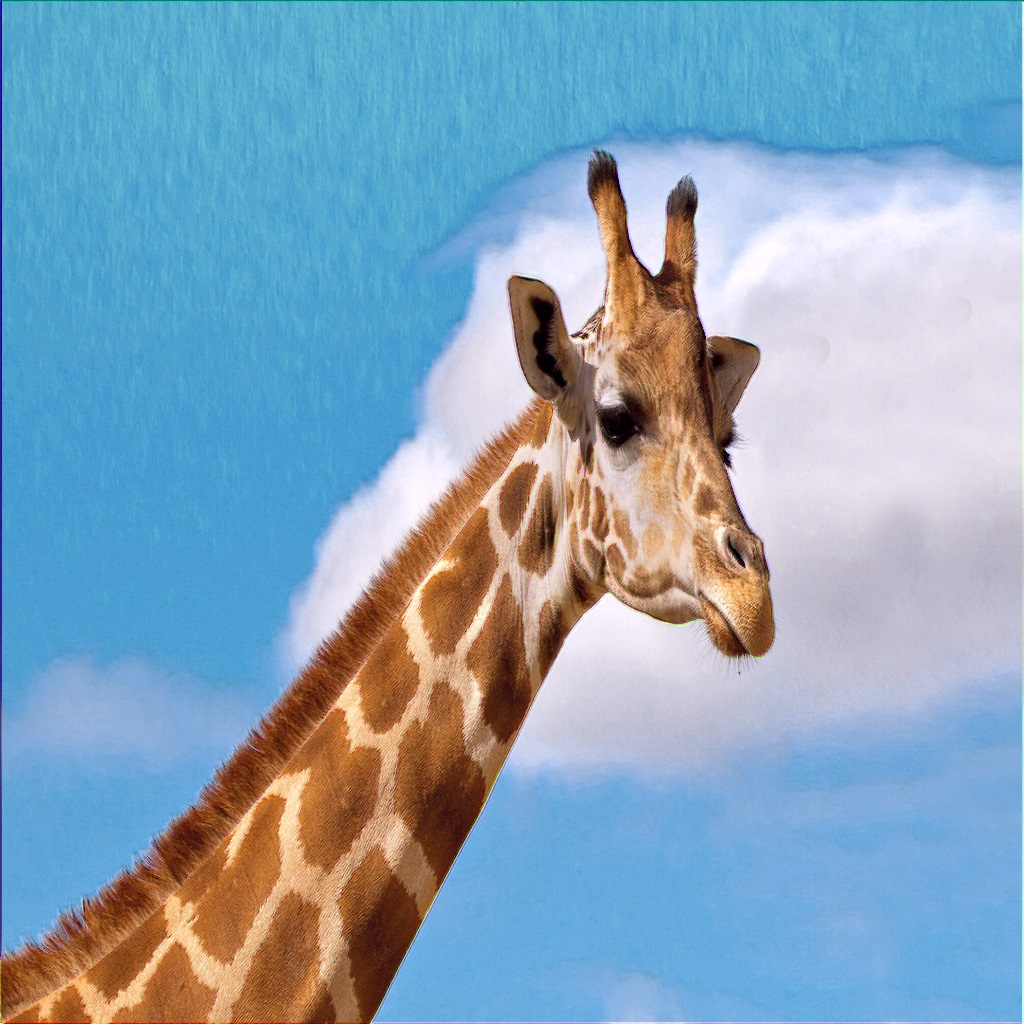
\includegraphics[width=\linewidth]{reconst_exper/dec_giraffe_my_1_test.jpg} % our reconstruction arc1 num.1	
	\end{subfigure}
	\begin{subfigure}[b]{0.13\linewidth}
		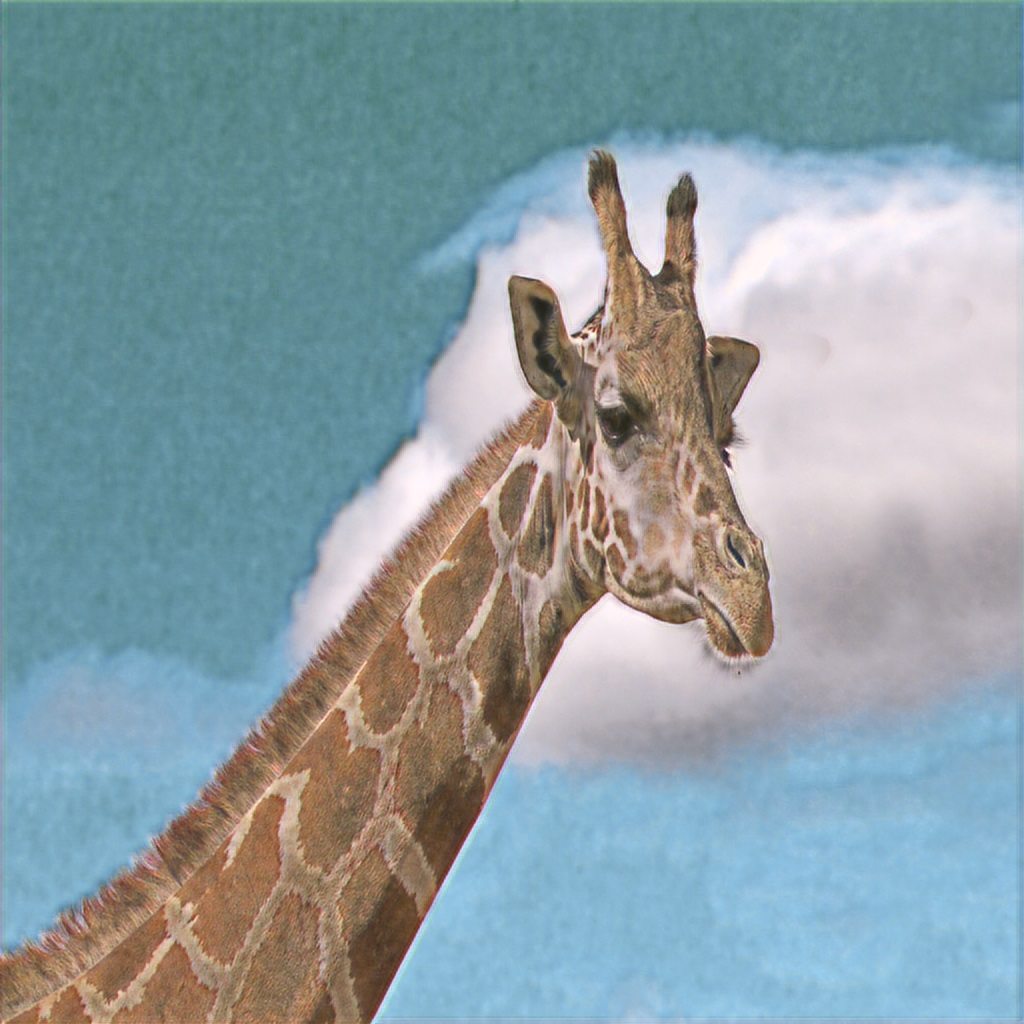
\includegraphics[width=\linewidth]{reconst_exper/dec_giraffe_my_2_test.jpg} % our reconstruction arc2 num.1	
	\end{subfigure}
	\begin{subfigure}[b]{0.13\linewidth}
		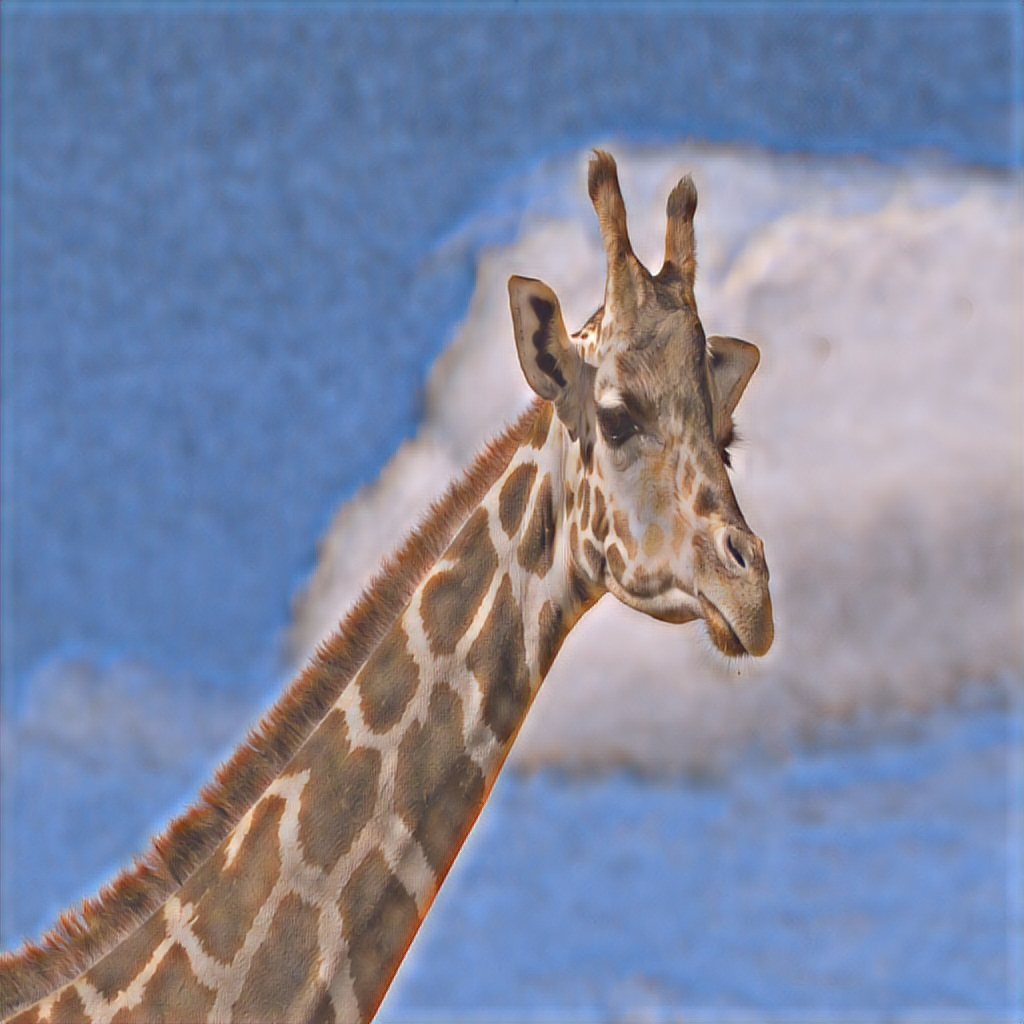
\includegraphics[width=\linewidth]{reconst_exper/dec_giraffe_my_3_test.jpg} % our reconstruction arc3 num.1	
	\end{subfigure}
	\begin{subfigure}[b]{0.13\linewidth}
		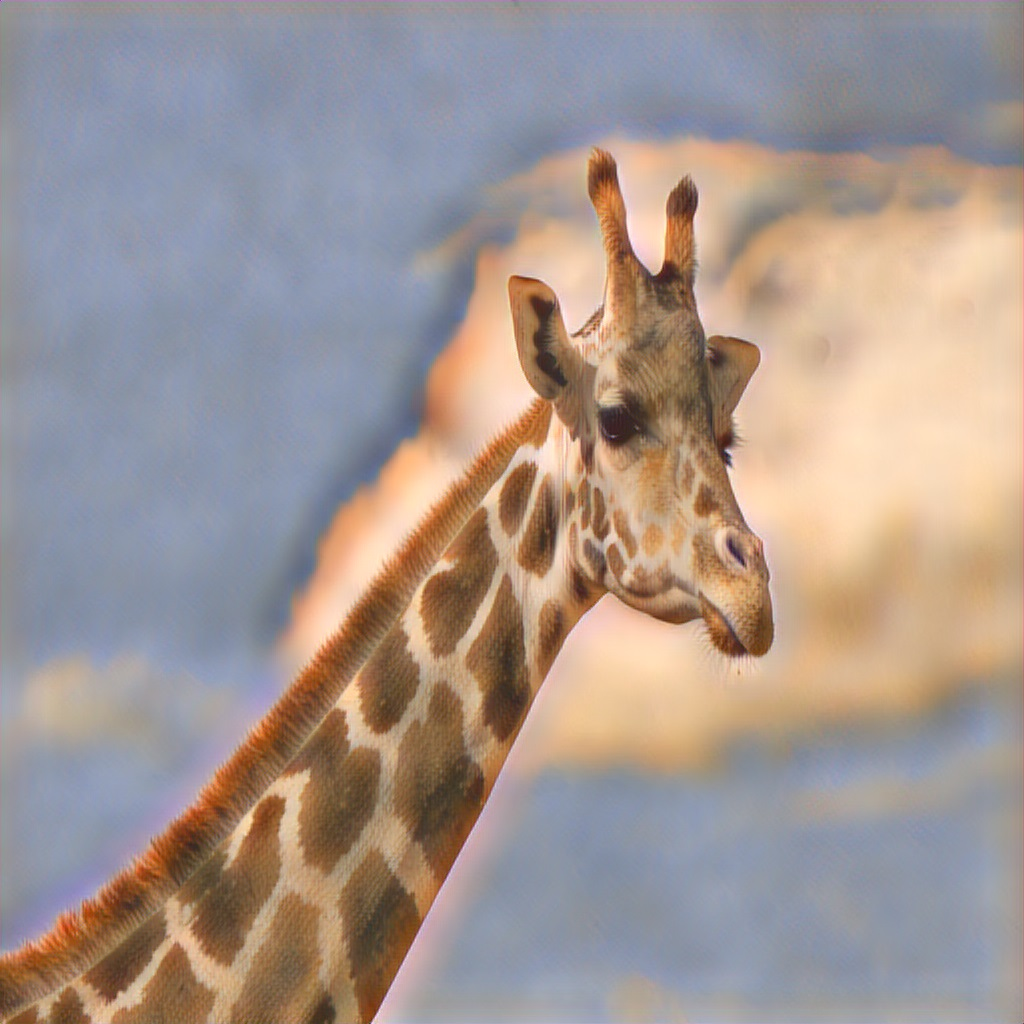
\includegraphics[width=\linewidth]{reconst_exper/dec_giraffe_my_4_test.jpg} % our reconstruction arc4 num.1	
	\end{subfigure}
	\begin{subfigure}[b]{0.13\linewidth}
		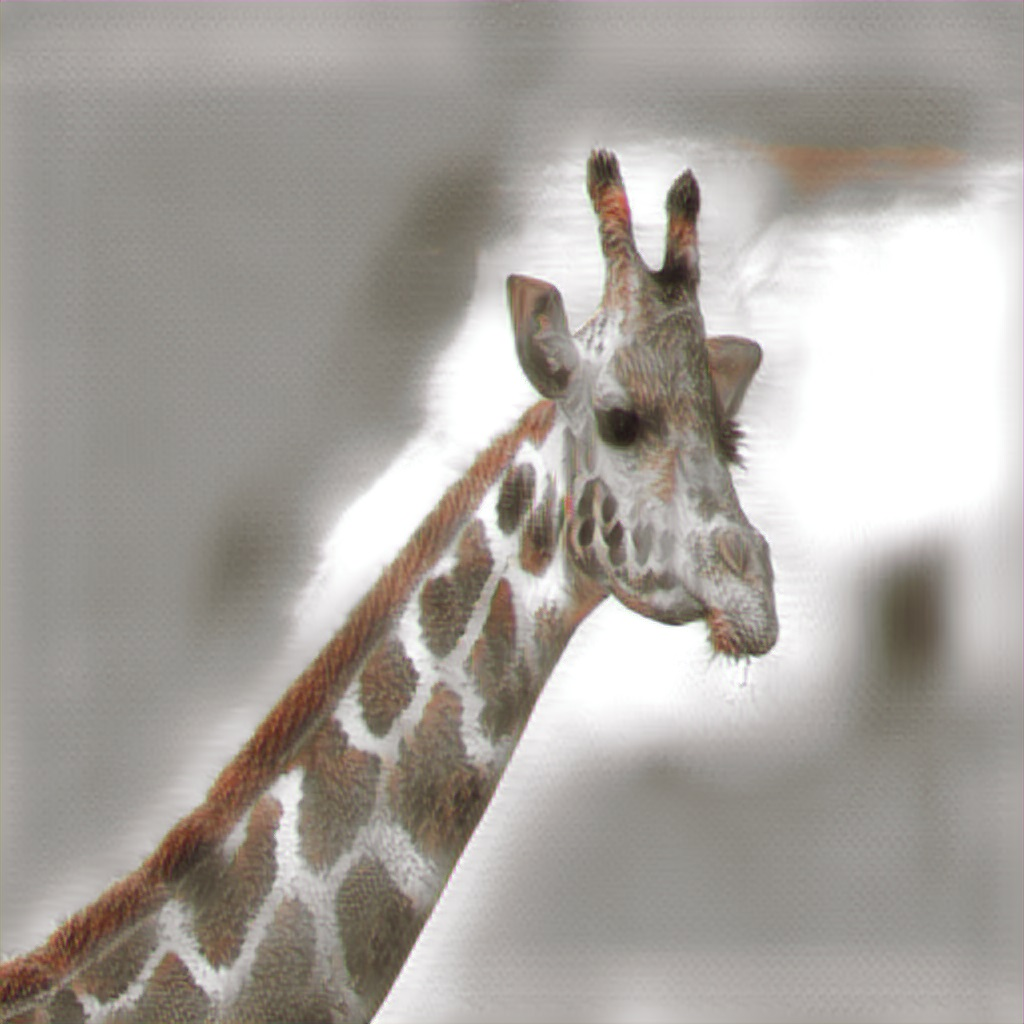
\includegraphics[width=\linewidth]{reconst_exper/dec_giraffe_my_5_test.jpg} % our reconstruction arc5 num.1	
	\end{subfigure}
	\begin{subfigure}[b]{0.13\linewidth}
		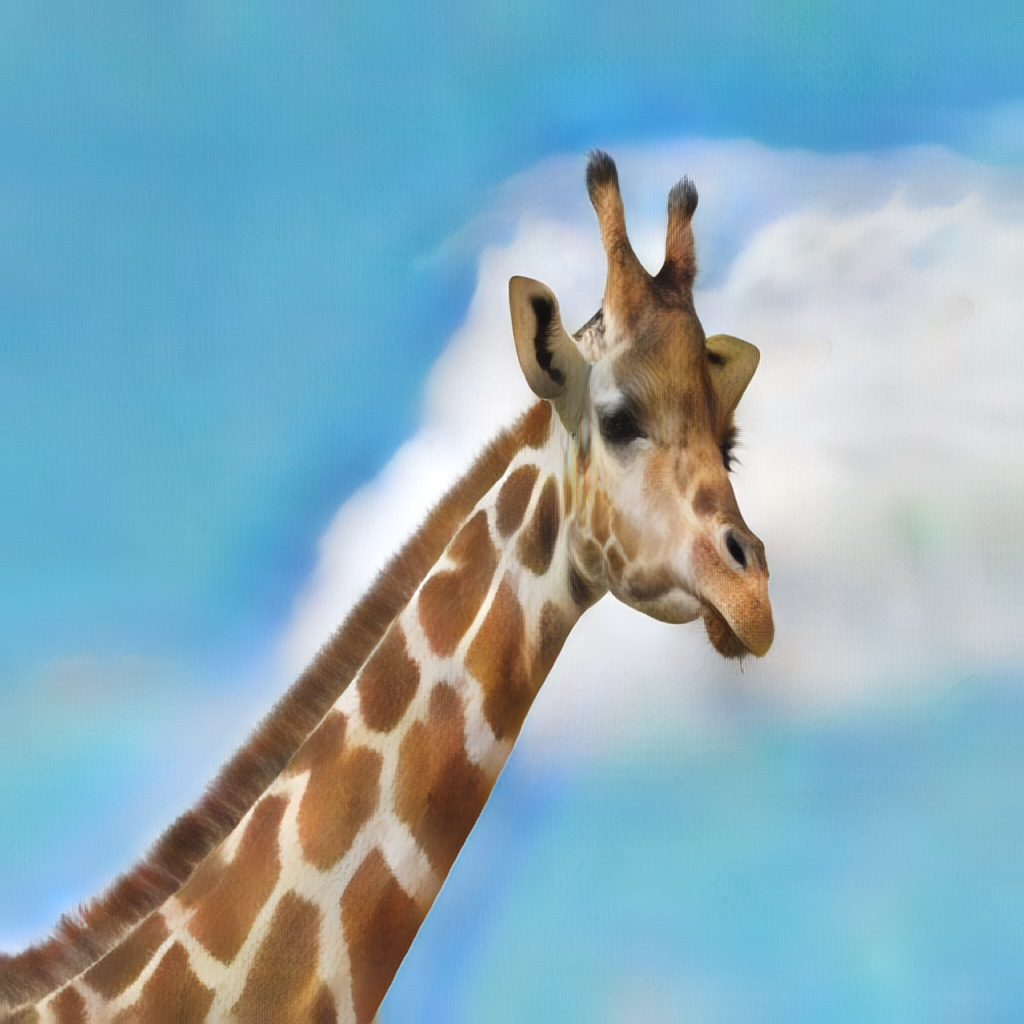
\includegraphics[width=\linewidth]{reconst_exper/dec_giraffe_ref_5_test.jpg} % their reconstruction arc5 num.1	
	\end{subfigure}
	% third line
	\centering
	\begin{subfigure}[b]{0.13\linewidth}
		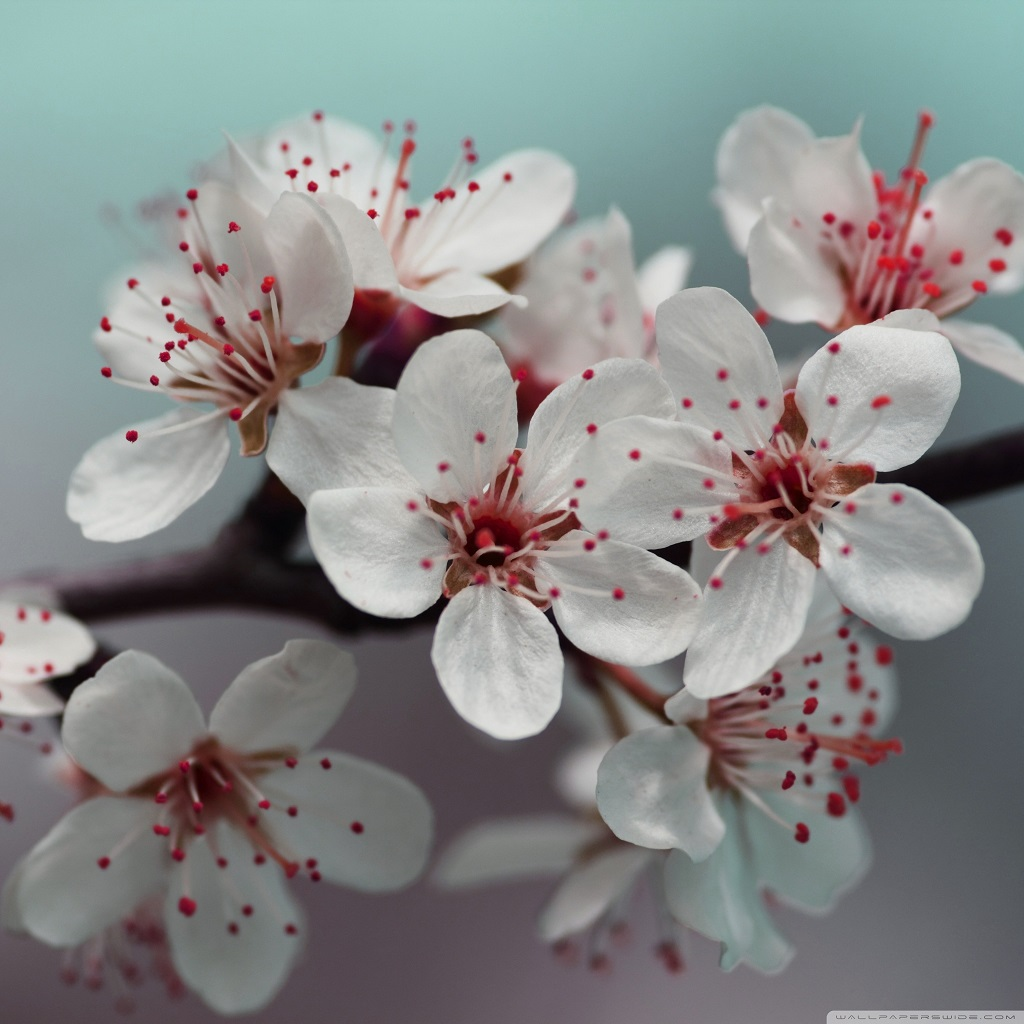
\includegraphics[width=\linewidth]{in1_sq.jpg} % original num.1	
	\end{subfigure}
	\begin{subfigure}[b]{0.13\linewidth}
		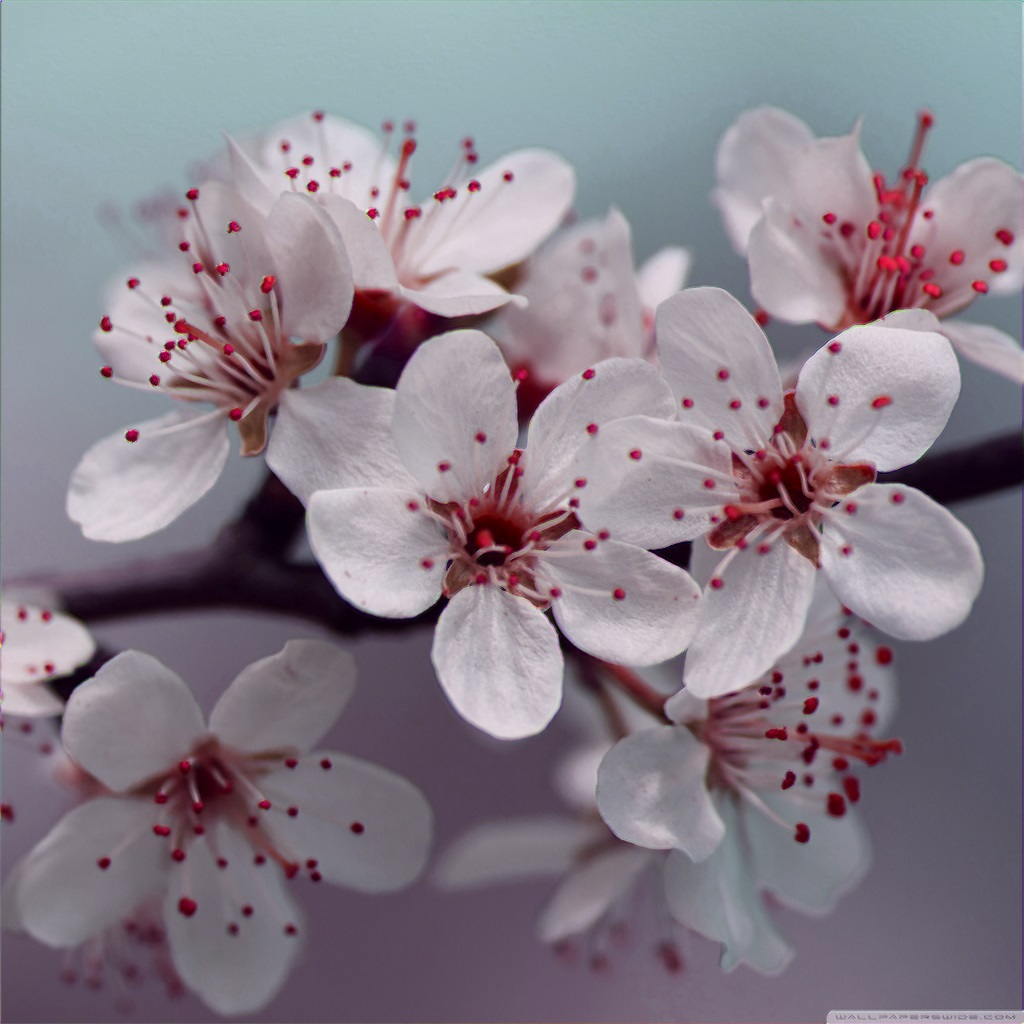
\includegraphics[width=\linewidth]{reconst_exper/dec_in1_my_1_test.jpg} % our reconstruction arc1 num.1	
	\end{subfigure}
	\begin{subfigure}[b]{0.13\linewidth}
		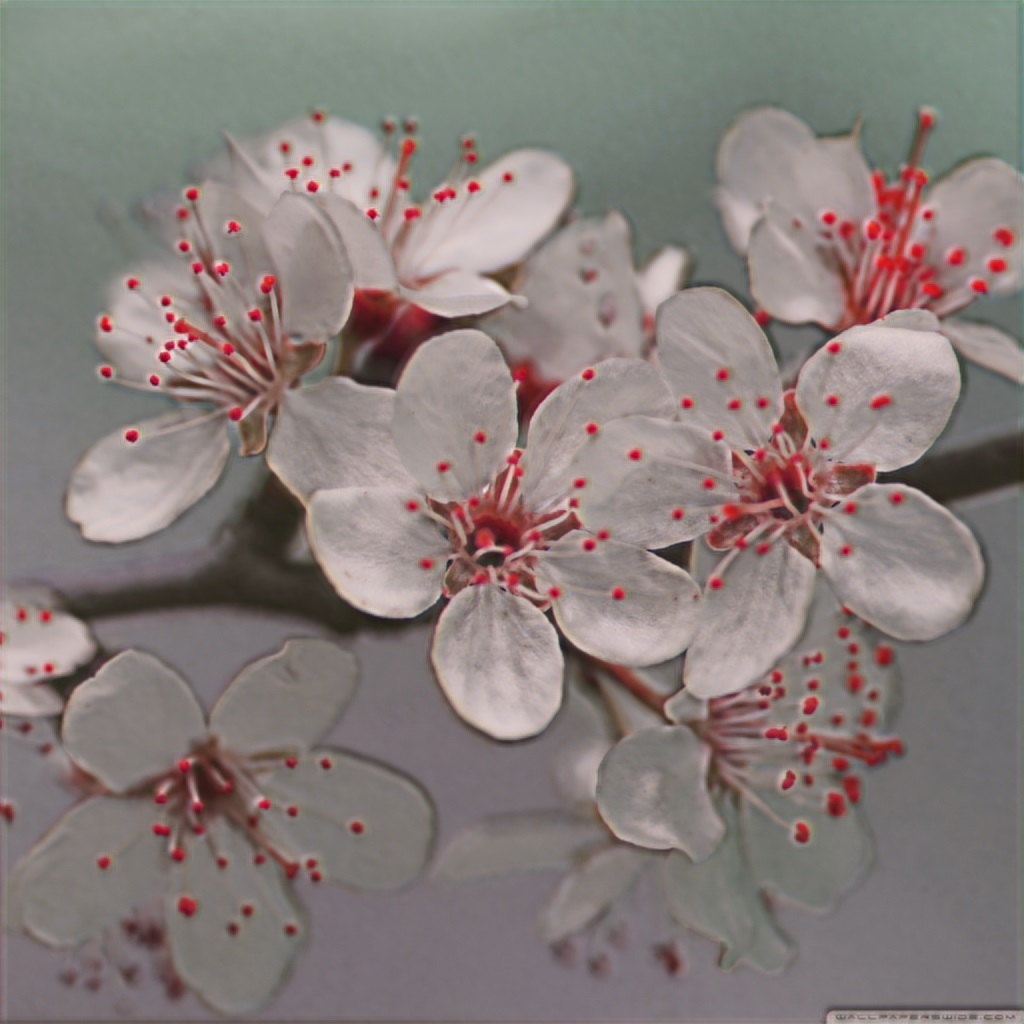
\includegraphics[width=\linewidth]{reconst_exper/dec_in1_my_2_test.jpg} % our reconstruction arc2 num.1	
	\end{subfigure}
	\begin{subfigure}[b]{0.13\linewidth}
		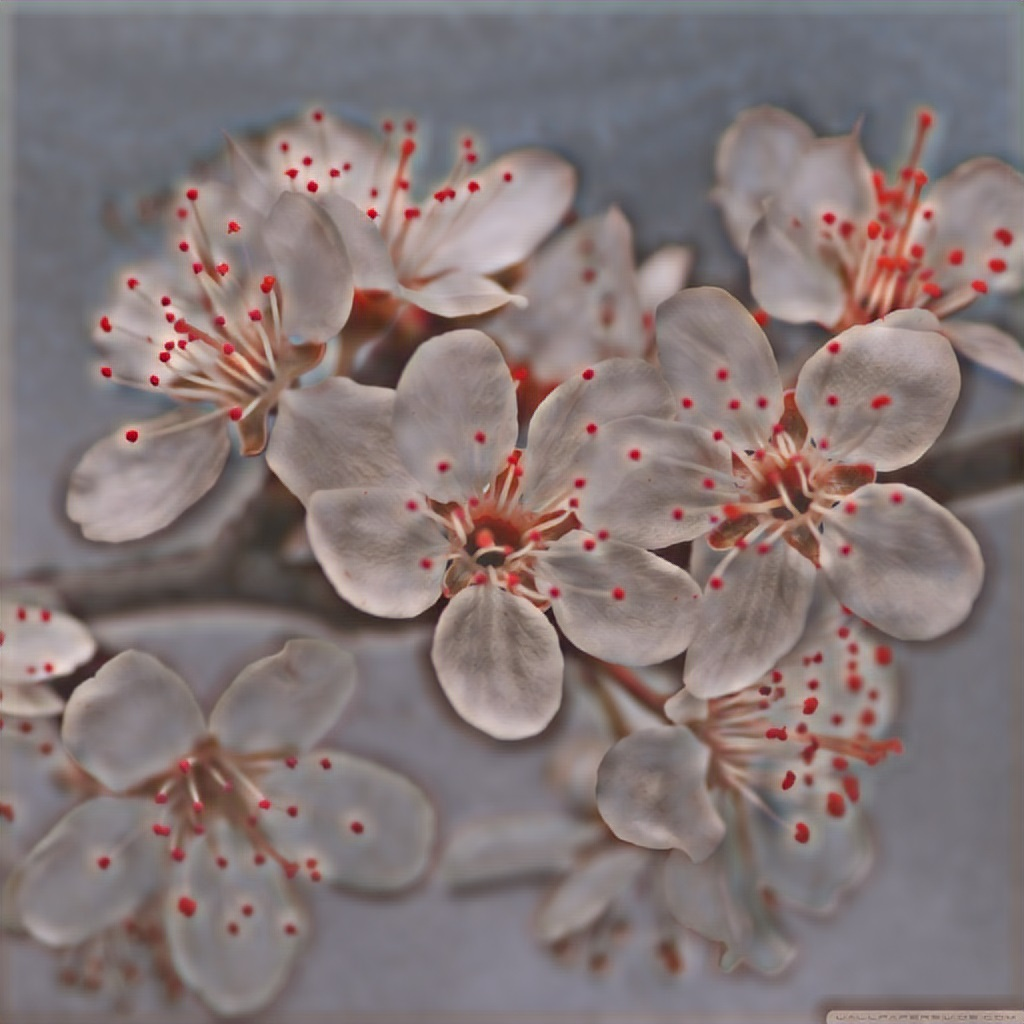
\includegraphics[width=\linewidth]{reconst_exper/dec_in1_my_3_test.jpg} % our reconstruction arc3 num.1	
	\end{subfigure}
	\begin{subfigure}[b]{0.13\linewidth}
		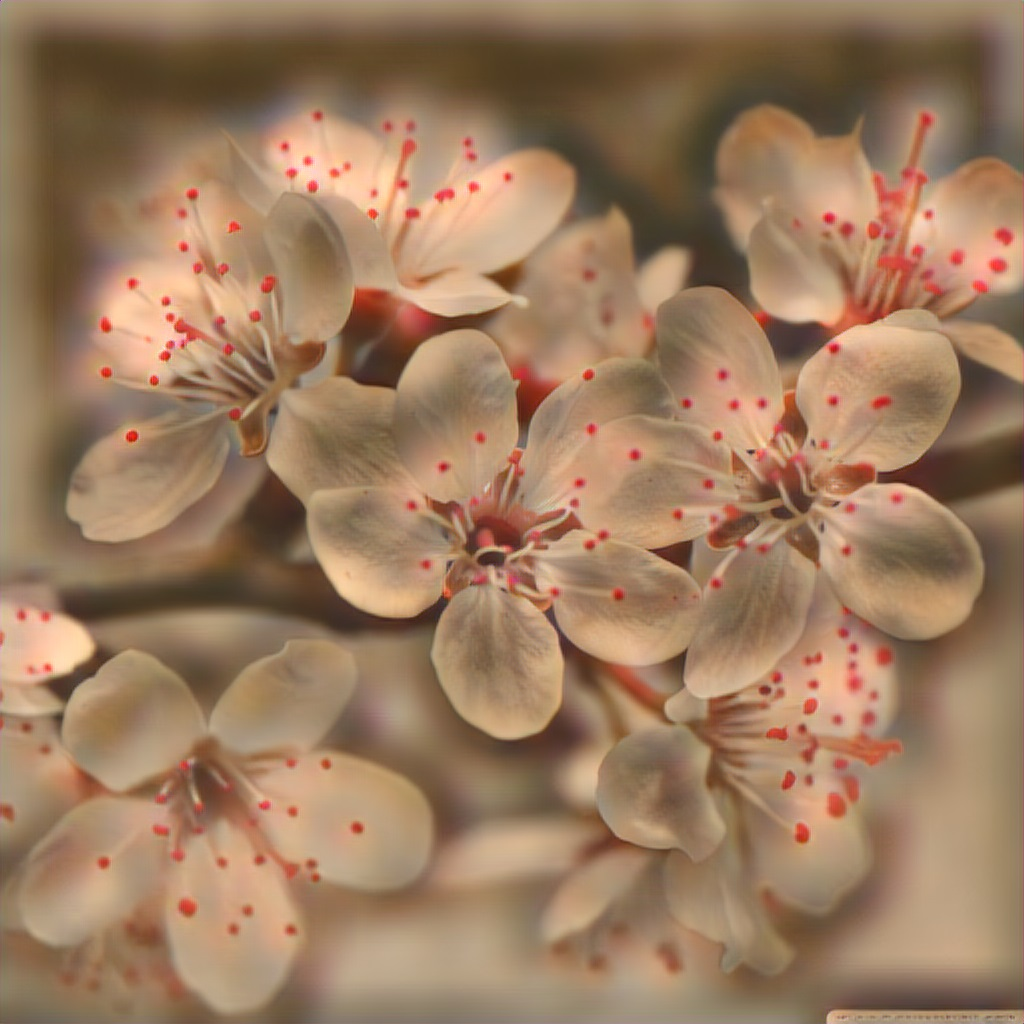
\includegraphics[width=\linewidth]{reconst_exper/dec_in1_my_4_test.jpg} % our reconstruction arc4 num.1	
	\end{subfigure}
	\begin{subfigure}[b]{0.13\linewidth}
		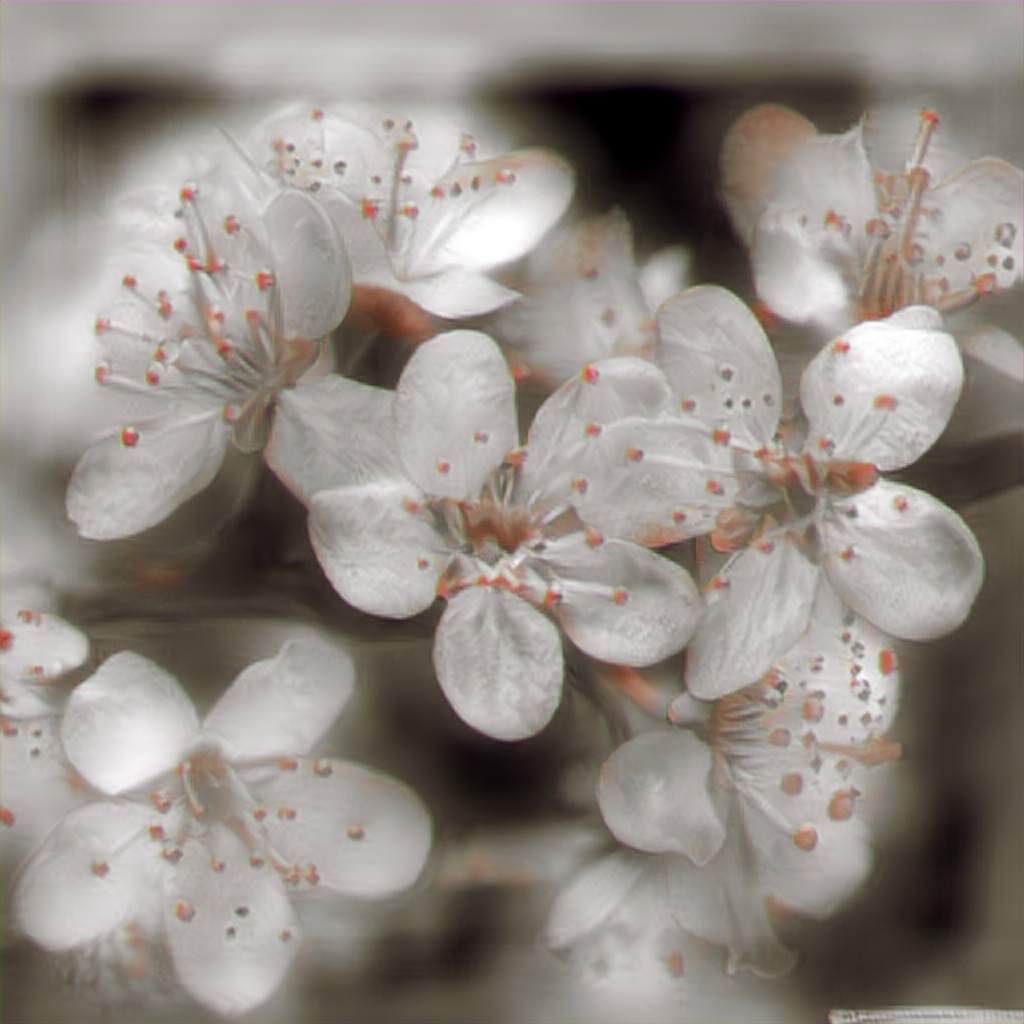
\includegraphics[width=\linewidth]{reconst_exper/dec_in1_my_5_test.jpg} % our reconstruction arc5 num.1	
	\end{subfigure}
	\begin{subfigure}[b]{0.13\linewidth}
		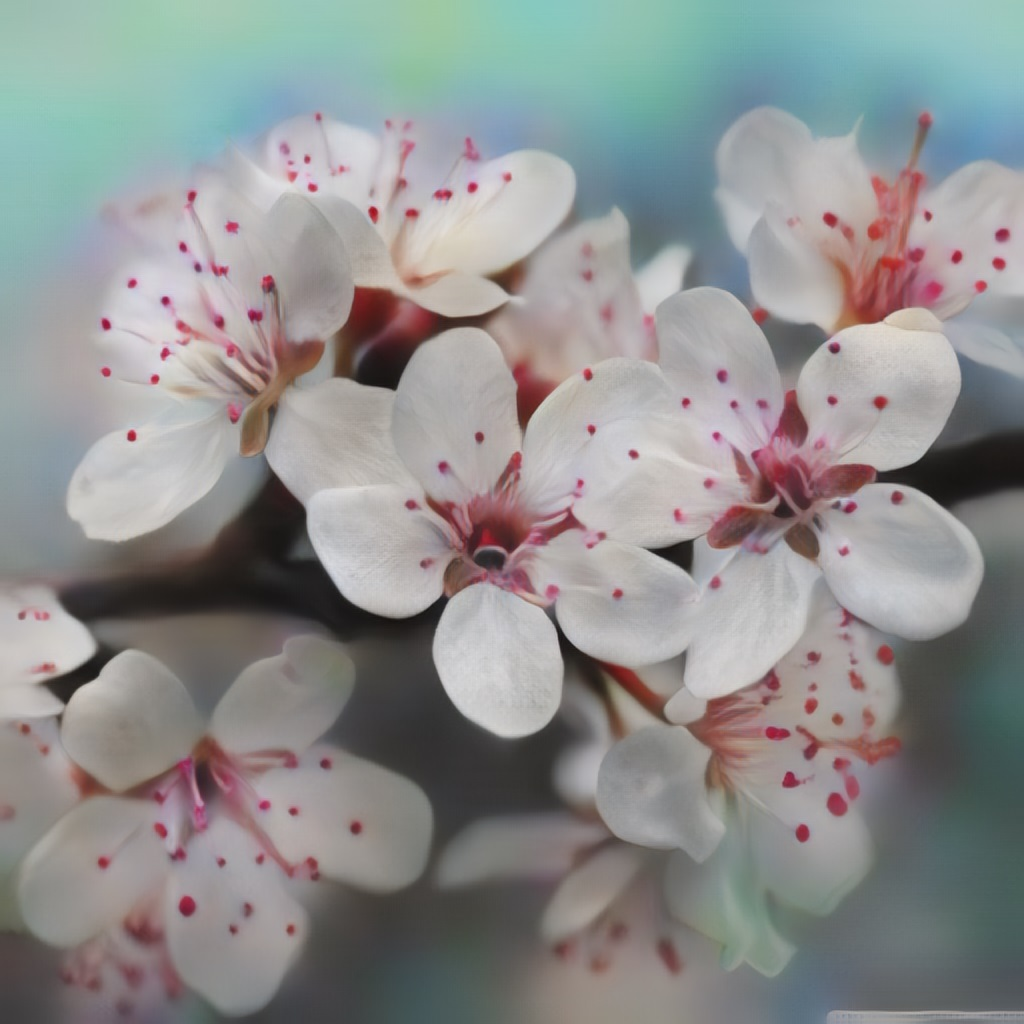
\includegraphics[width=\linewidth]{reconst_exper/dec_in1_ref_5_test.jpg} % their reconstruction arc5 num.1	
	\end{subfigure}
	%fourth line
	\centering
	\begin{subfigure}[b]{0.13\linewidth}
		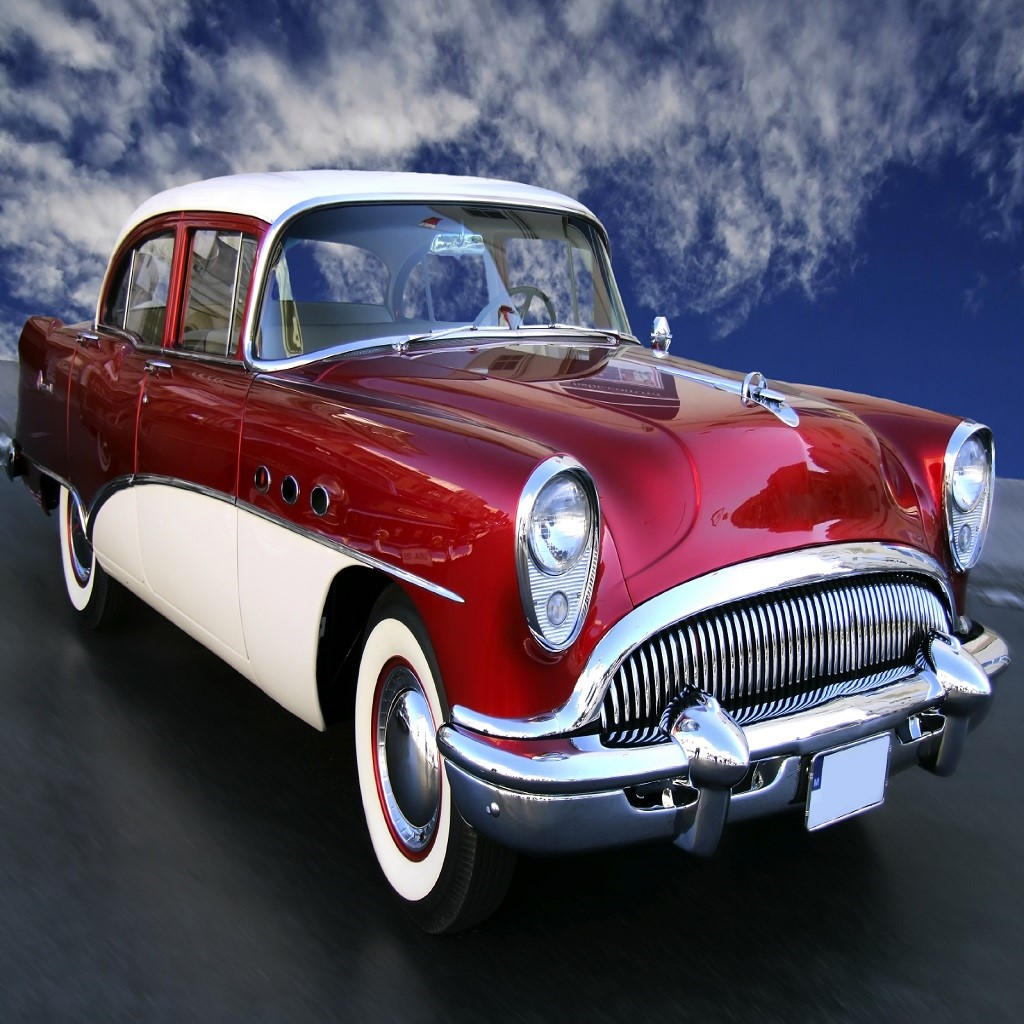
\includegraphics[width=\linewidth]{car_sq.jpg} % original num.1	
	\end{subfigure}
	\begin{subfigure}[b]{0.13\linewidth}
		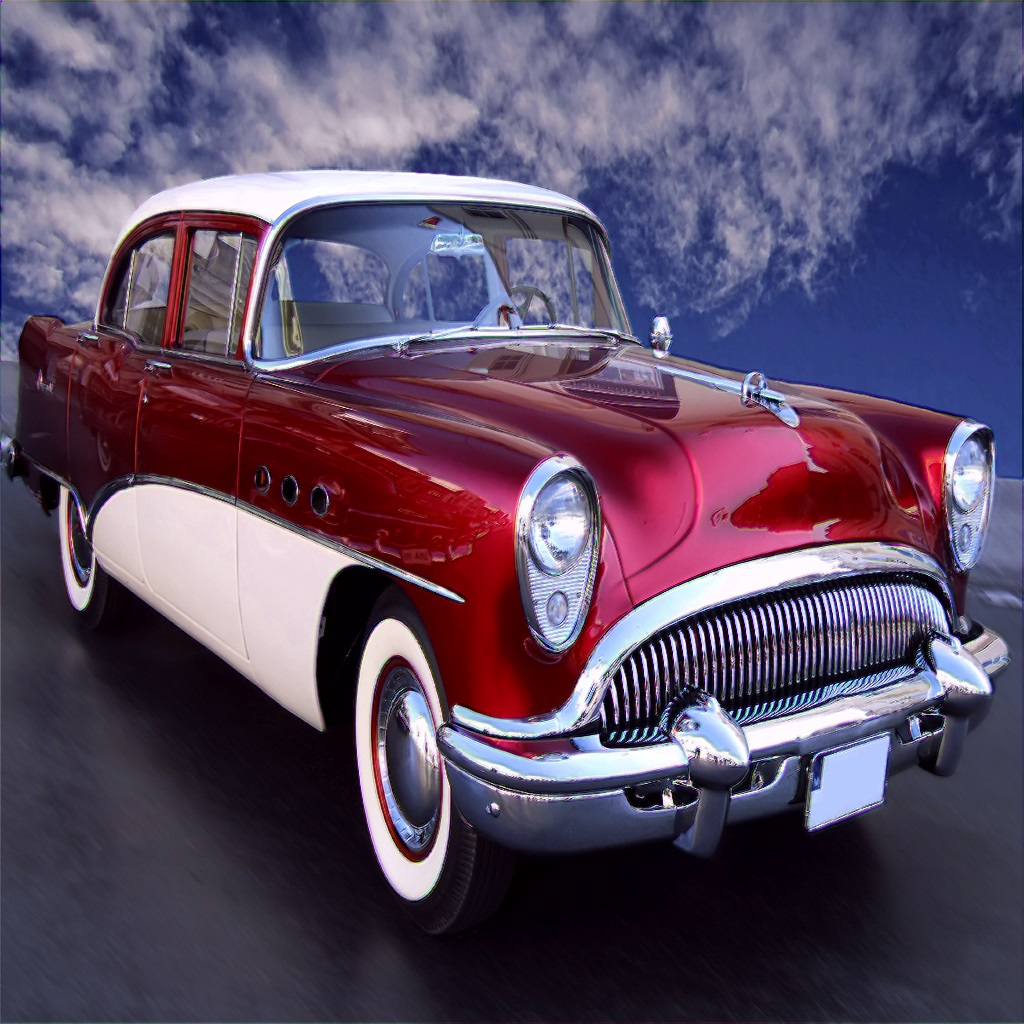
\includegraphics[width=\linewidth]{reconst_exper/dec_in2_my_1_test.jpg} % our reconstruction arc1 num.1	
	\end{subfigure}
	\begin{subfigure}[b]{0.13\linewidth}
		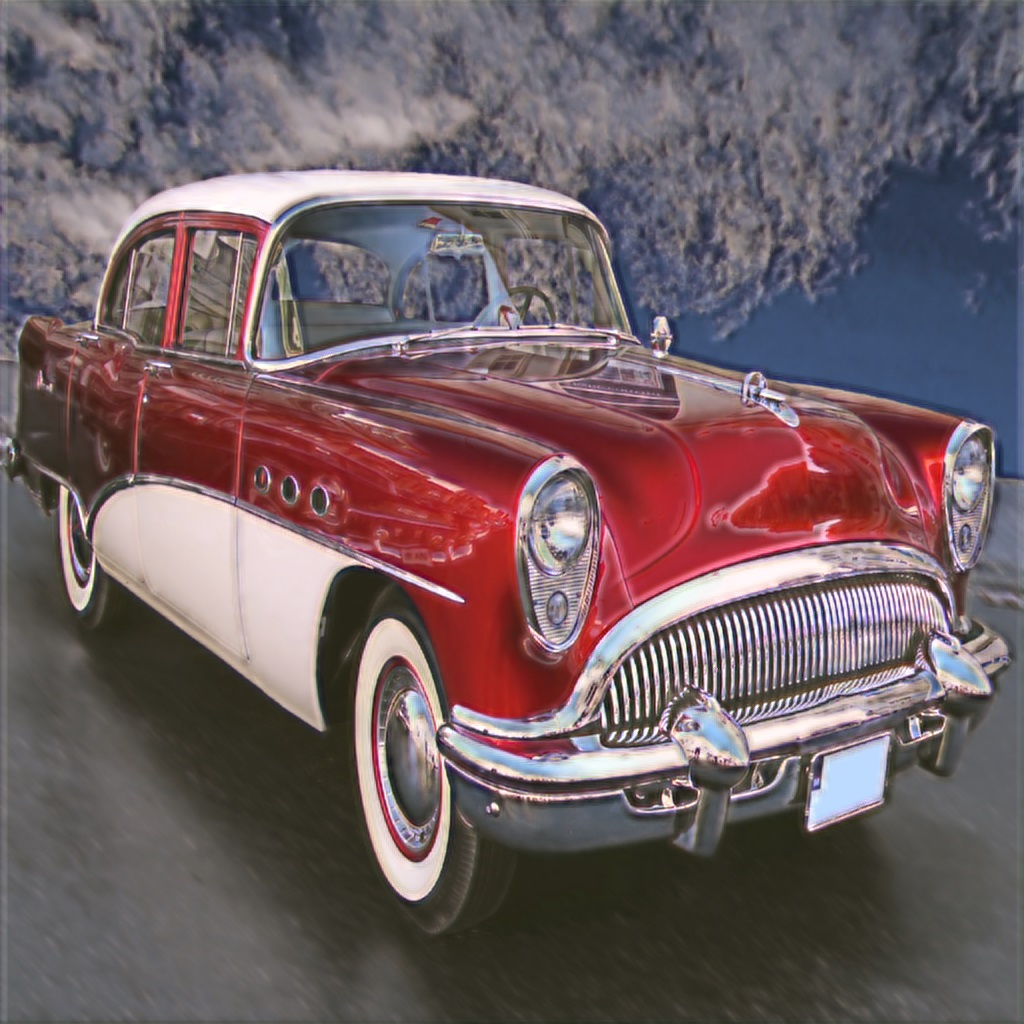
\includegraphics[width=\linewidth]{reconst_exper/dec_in2_my_2_test.jpg} % our reconstruction arc2 num.1	
	\end{subfigure}
	\begin{subfigure}[b]{0.13\linewidth}
		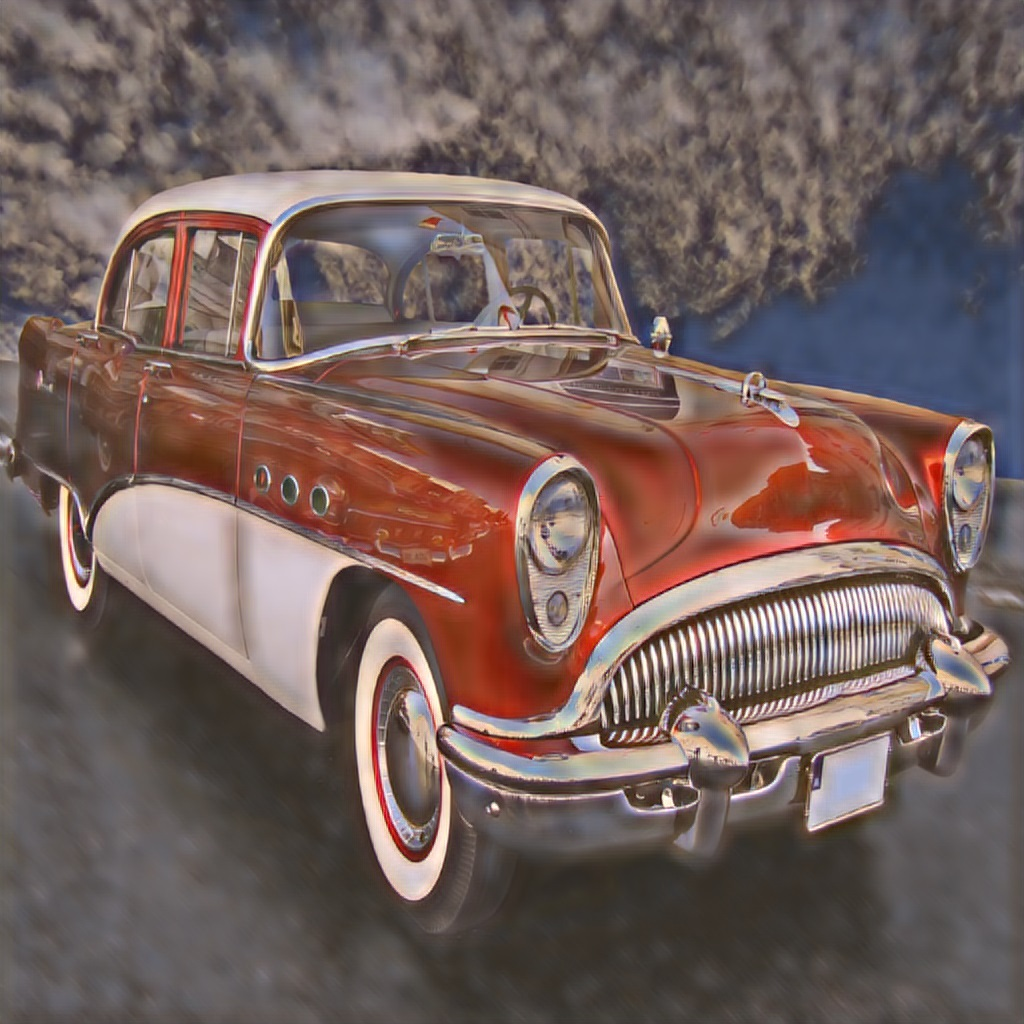
\includegraphics[width=\linewidth]{reconst_exper/dec_in2_my_3_test.jpg} % our reconstruction arc3 num.1	
	\end{subfigure}
	\begin{subfigure}[b]{0.13\linewidth}
		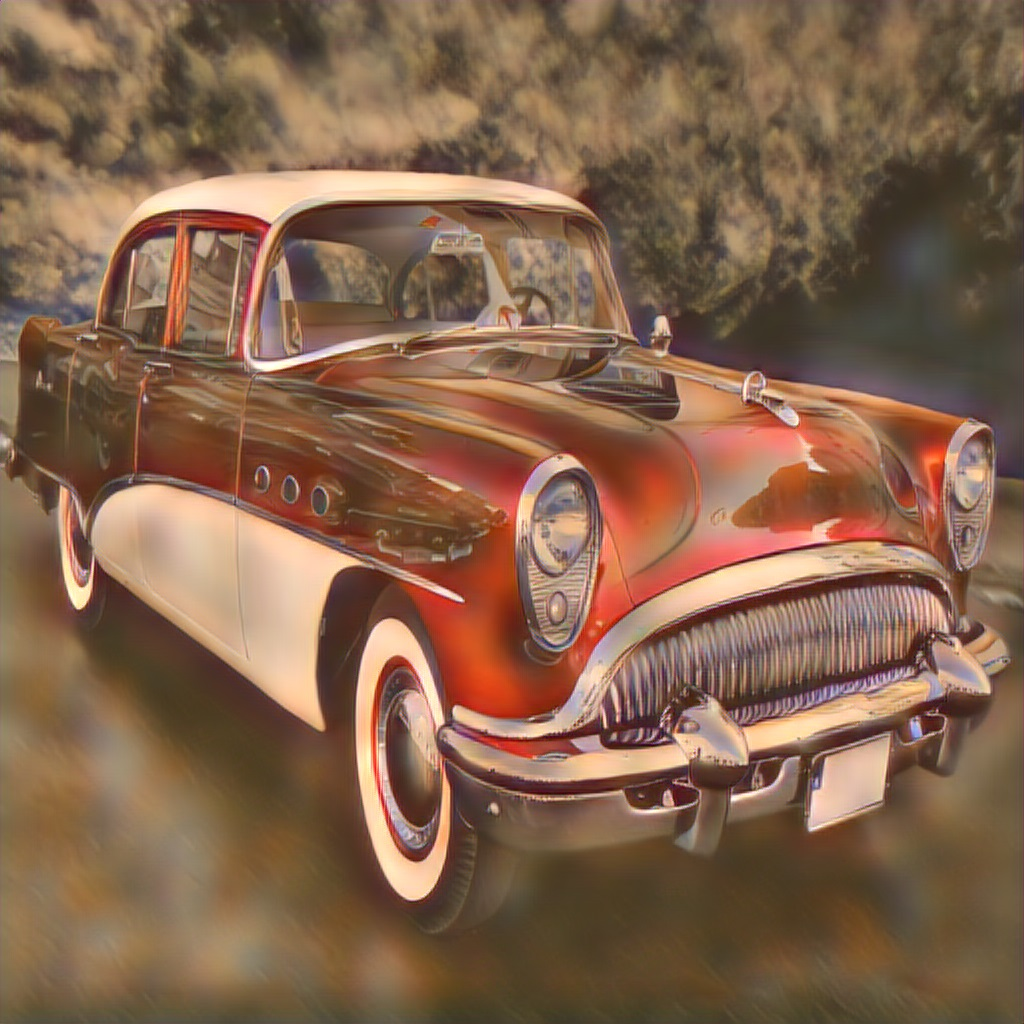
\includegraphics[width=\linewidth]{reconst_exper/dec_in2_my_4_test.jpg} % our reconstruction arc4 num.1	
	\end{subfigure}
	\begin{subfigure}[b]{0.13\linewidth}
		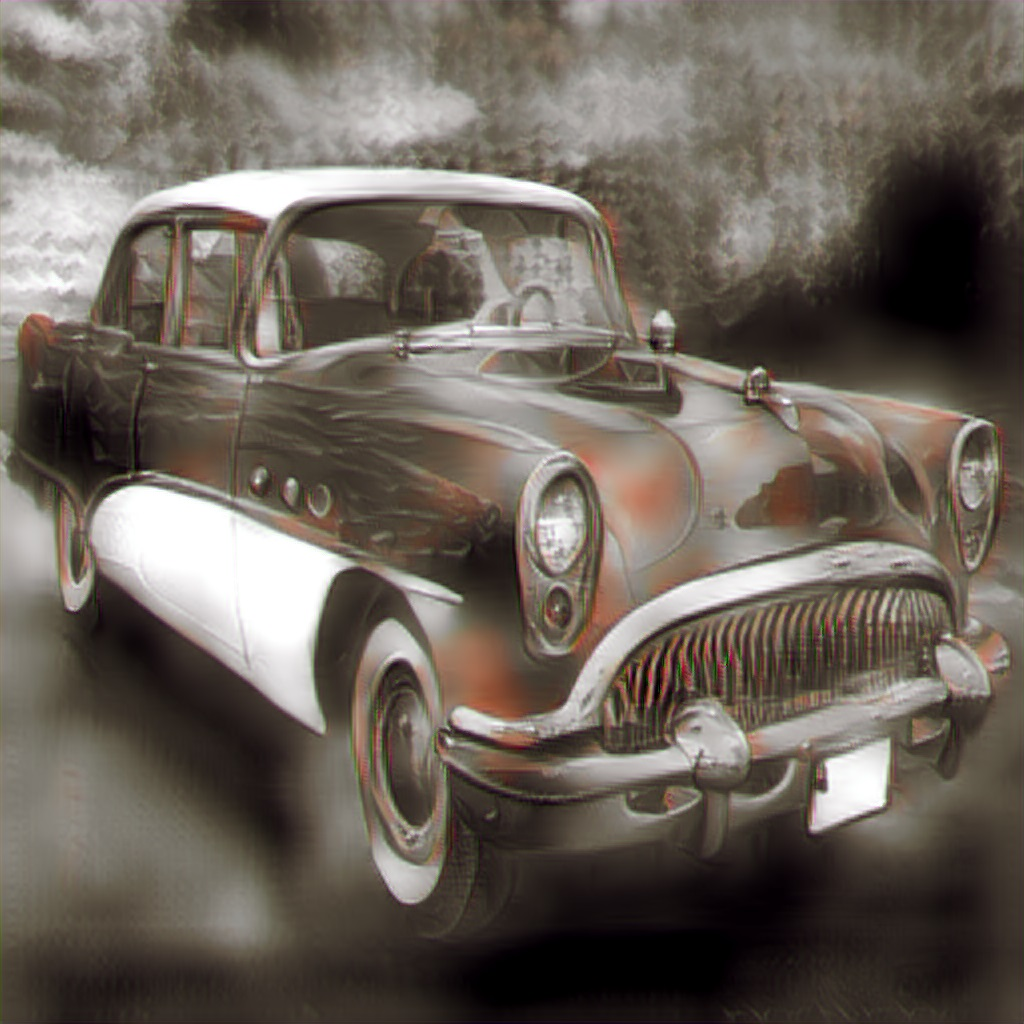
\includegraphics[width=\linewidth]{reconst_exper/dec_in2_my_5_test.jpg} % our reconstruction arc5 num.1	
	\end{subfigure}
	\begin{subfigure}[b]{0.13\linewidth}
		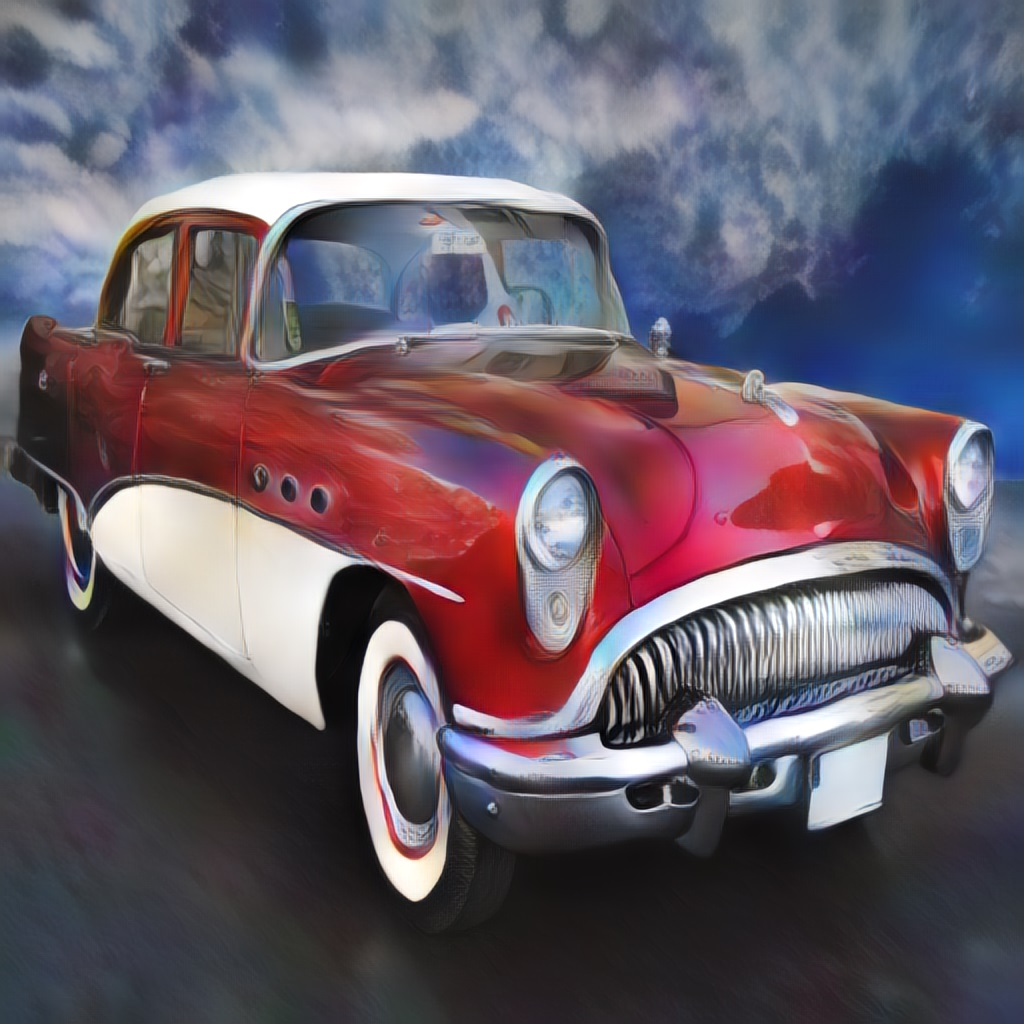
\includegraphics[width=\linewidth]{reconst_exper/dec_in2_ref_5_test.jpg} % their reconstruction arc5 num.1	
	\end{subfigure}
	% fifth line
	\centering
	\begin{subfigure}[b]{0.13\linewidth}
		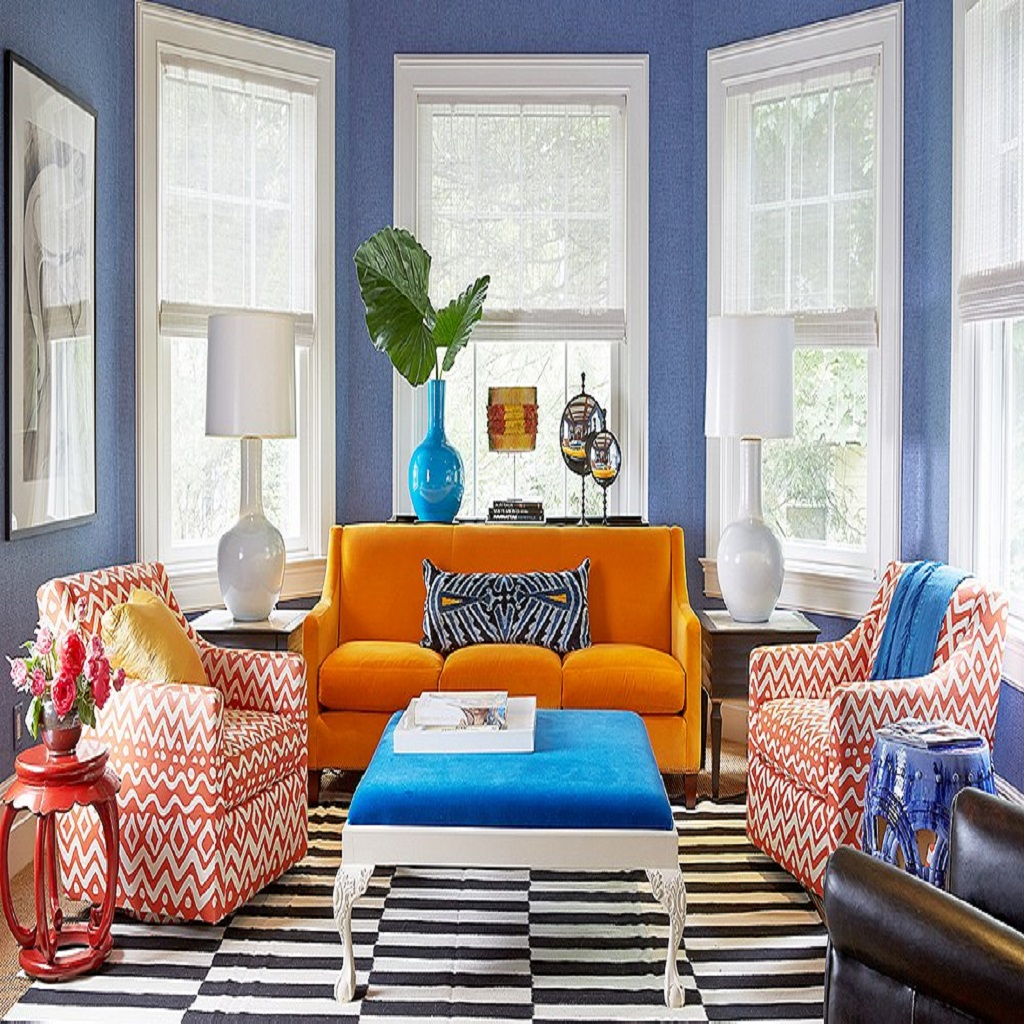
\includegraphics[width=\linewidth]{room_sq.jpg} % original num.5
		\caption{Original}
	\end{subfigure}
	\begin{subfigure}[b]{0.13\linewidth}
		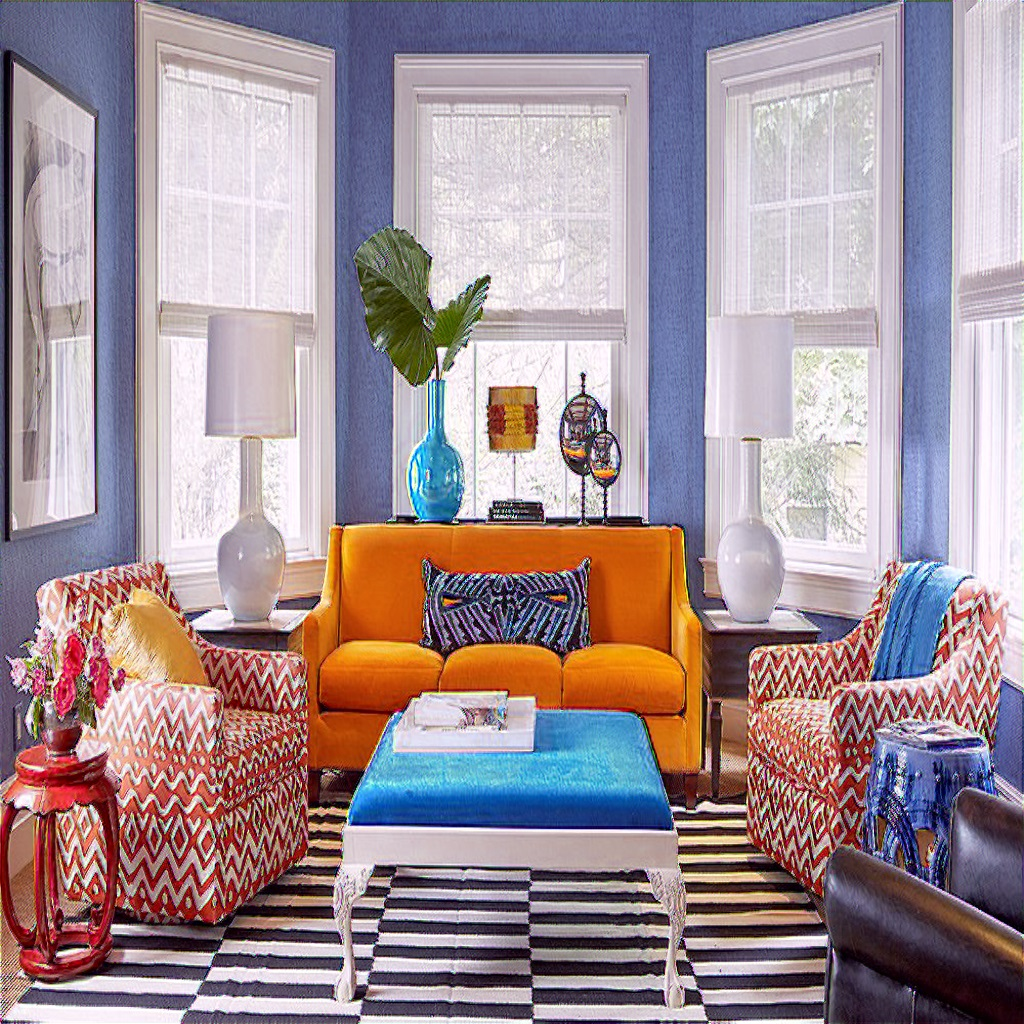
\includegraphics[width=\linewidth]{reconst_exper/dec_room_my_1_test.jpg} % our reconstruction num.5
		\caption{Ours arc1}
	\end{subfigure}
	\begin{subfigure}[b]{0.13\linewidth}
		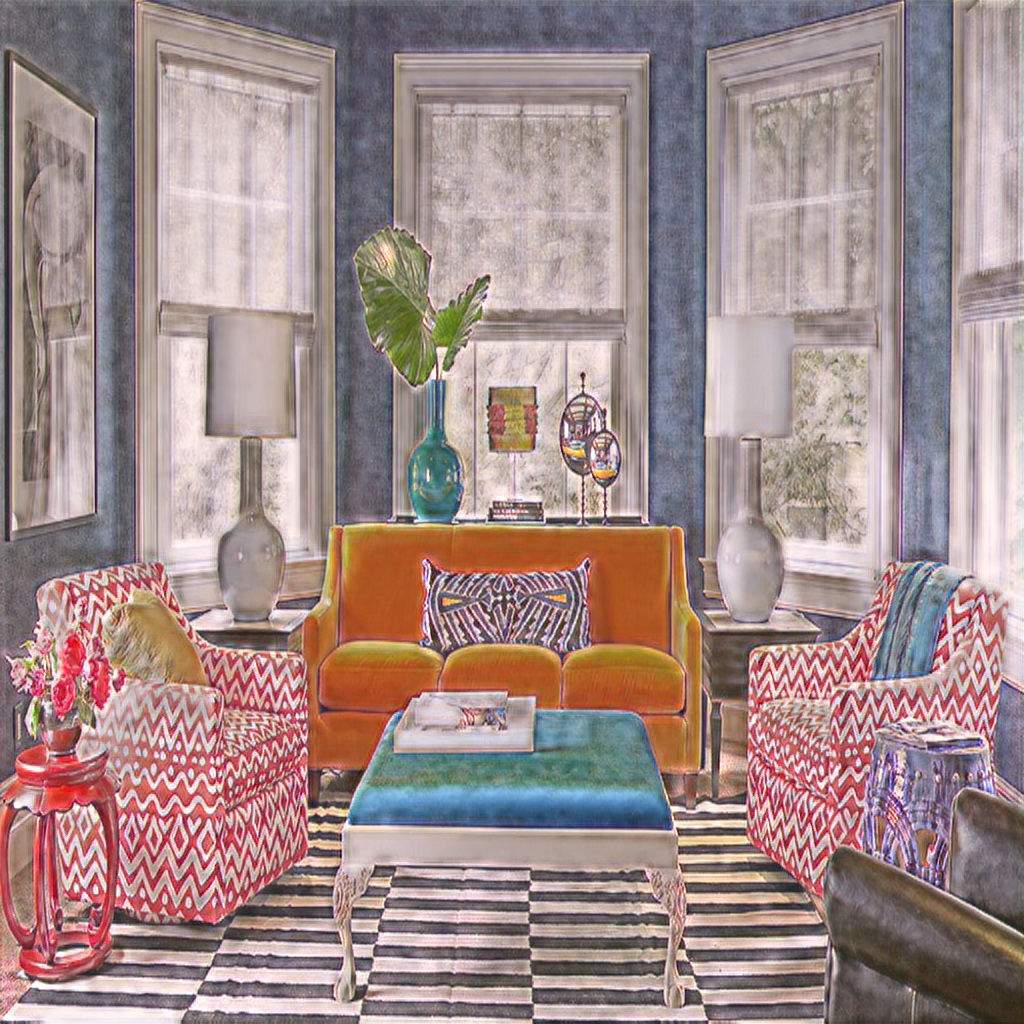
\includegraphics[width=\linewidth]{reconst_exper/dec_room_my_2_test.jpg} % our reconstruction num.5
		\caption{Ours arc2}
	\end{subfigure}
	\begin{subfigure}[b]{0.13\linewidth}
		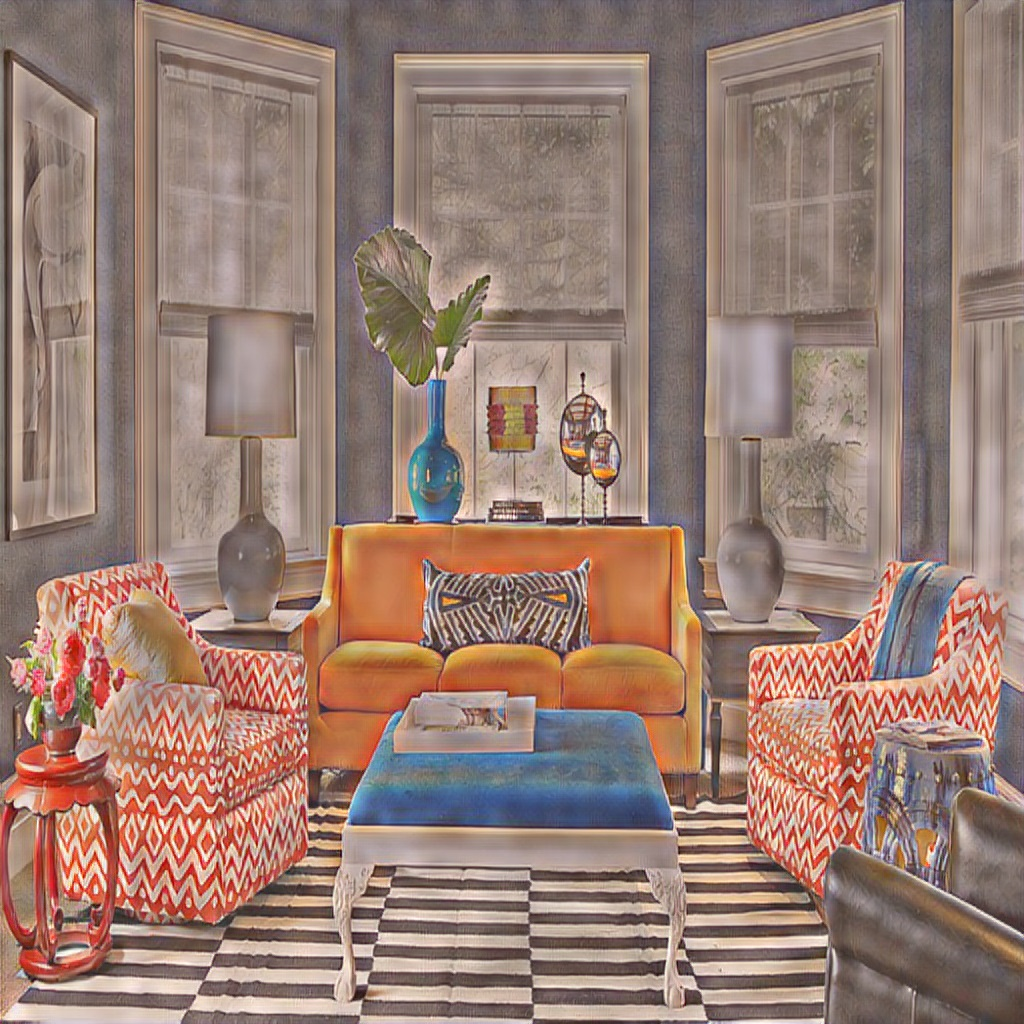
\includegraphics[width=\linewidth]{reconst_exper/dec_room_my_3_test.jpg} % our reconstruction num.5
		\caption{Ours arc3}
	\end{subfigure}
	\begin{subfigure}[b]{0.13\linewidth}
		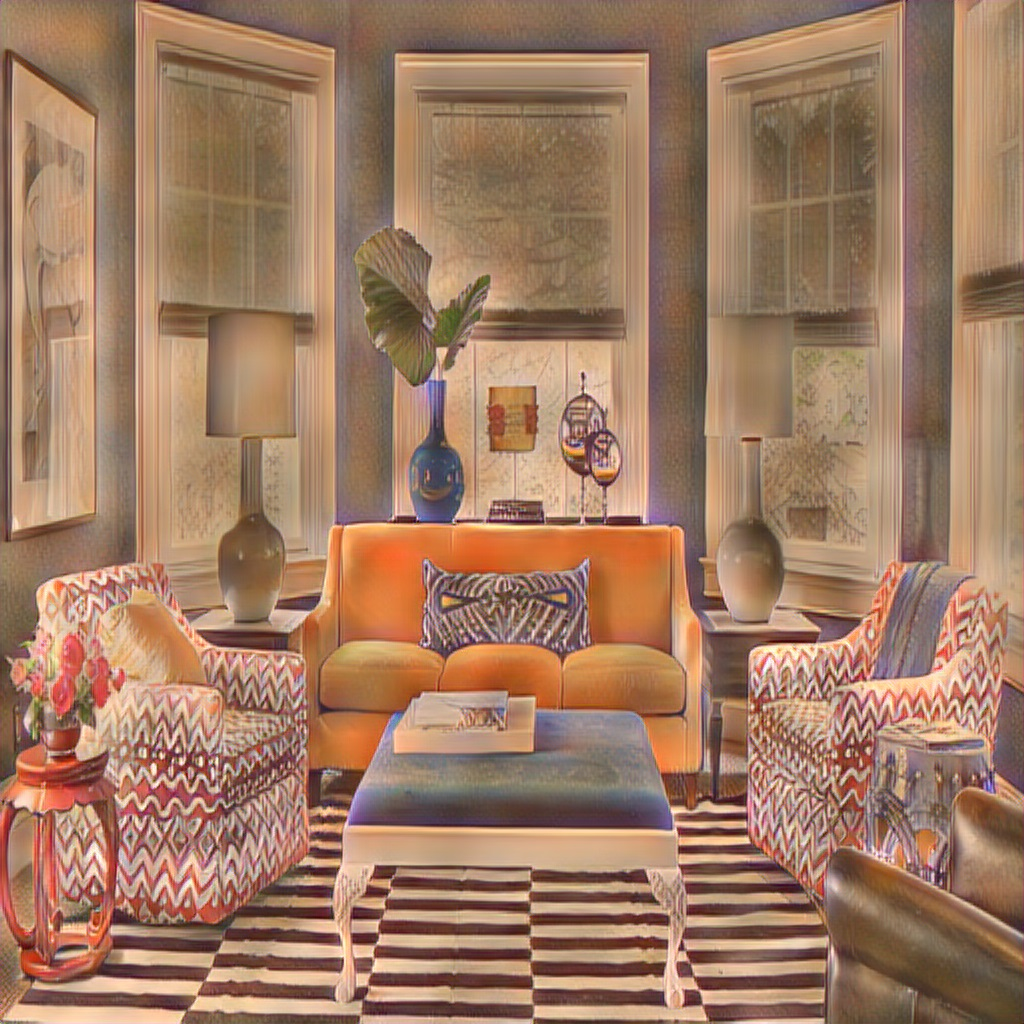
\includegraphics[width=\linewidth]{reconst_exper/dec_room_my_4_test.jpg} % our reconstruction num.5
		\caption{Ours arc4}
	\end{subfigure}
	\begin{subfigure}[b]{0.13\linewidth}
		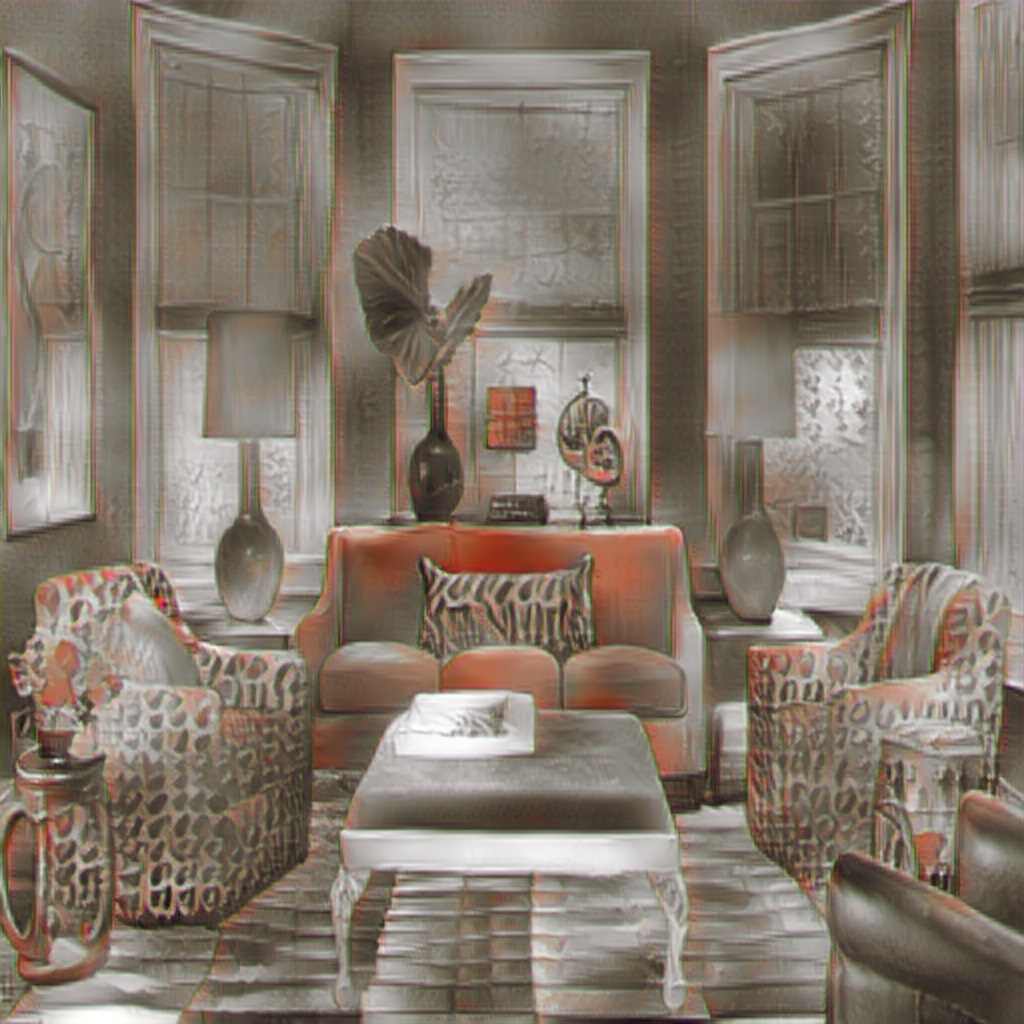
\includegraphics[width=\linewidth]{reconst_exper/dec_room_my_5_test.jpg} % our reconstruction num.5
		\caption{Ours arc5}
	\end{subfigure}
	\begin{subfigure}[b]{0.13\linewidth}
		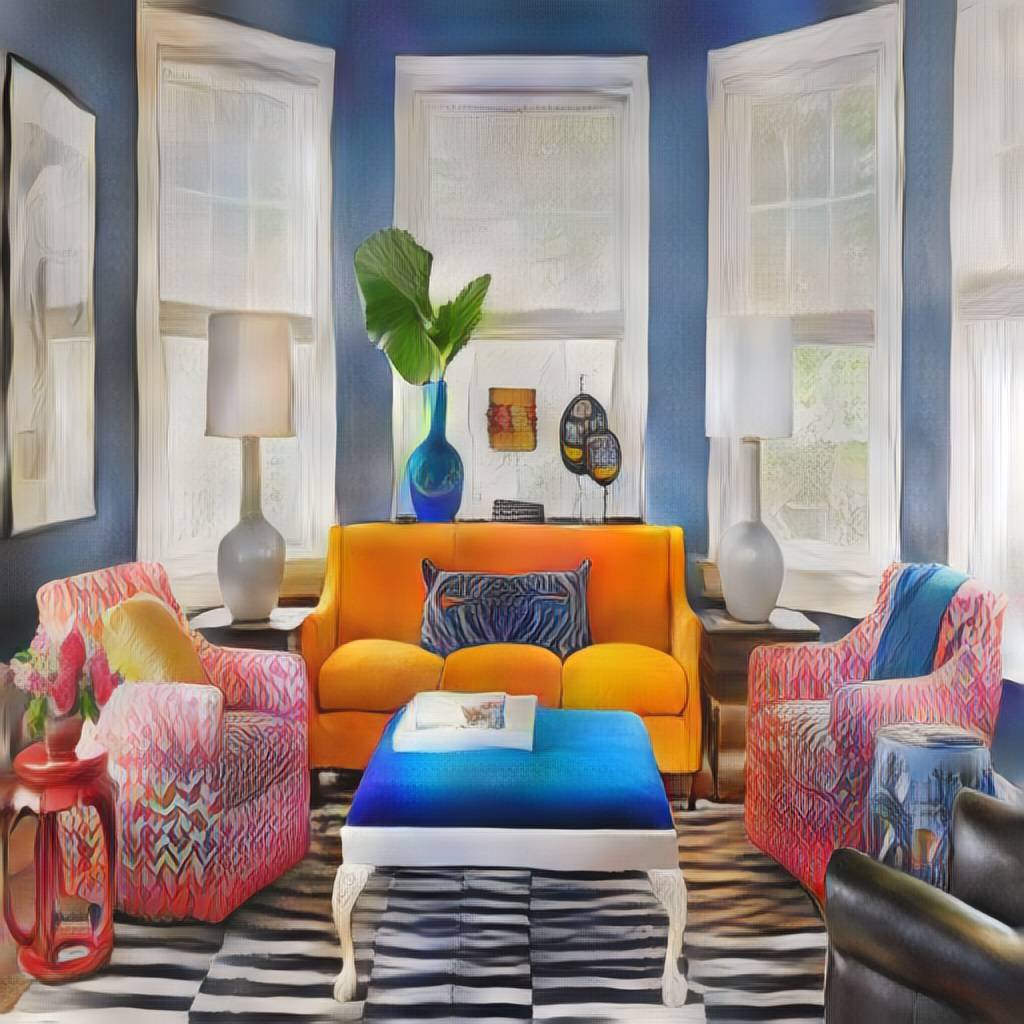
\includegraphics[width=\linewidth]{reconst_exper/dec_room_ref_5_test.jpg} % their reconstruction arc5 num.1
		\caption{Ref arc5}	
	\end{subfigure}
	\caption{Image Reconstruction in different architectures}
	\label{fig:reconstruction}
\end{figure}

\textcolor{red}{TODO: address the results from the numeric table} Our distortion-of-reconstruction loss table ~\ref{Tab:loss} shows by both pixel and feature loss, that the first architecture has the less loss since it is only uses 1 convolution layer. As we go deeper in architectures in a manner of convolutional layers, we see that the loss arises respectively.\\

From Figure ~\ref{fig:reconstruction} it can be seen that our architectures \#1-4 conserve the original image's color to some degree. Architecture \#5, unlike them, only preserves a fraction of the color tones originally available in the input - mostly some of the reds. Additionally, the deeper the architecture is, the more details are lost in the reconstruction process. Another problem is image regions going gray, and losing their contrast, such as the shade of the car in the fourth row or the blue walls in the fifth. Keeping in mind the trade-off between pipeline depth and image distortion, in order to get the best results possible from the models trained by us, we choose to shorten our pipeline such that it would consist of the four last pipeline levels from ~\ref{fig:style_transfer}. In this way we expect our pipeline to produce good reconstruction quality as well as use deep enough features while transferring style. This means we leave architecture \#5 unused when transferring style using our trained models.\\
These visual results show that our models are not sufficiently trained. The main difficulty in training these models was a lack of compute power. The models, based on VGG-19 are relatively large and converge very slowly towards optimality. We strongly believe that given more powerful resources we could have trained better performing decoders.\\
\textcolor{red}{Consider making an experiment showing reconstruction through the pipeline 4321, next to style transfer or just next to the reference (justification for choosing 4321 as our pipeline)}
  
%%%%%%%%%%%%%%%%%%%%%%%%%%%%
%%%%%%%%%%%%%%%%%%%%%%%%%%%%
% style transfer images %
%%%%%%%%%%%%%%%%%%%%%%%%%%%%
%%%%%%%%%%%%%%%%%%%%%%%%%%%%

\subsection{Style Transfer Experimental Results}
This section display the results of our implementation of UST\cite{bib11}. Unlike the previous section where the images only when through reconstruction, this time we run the entire algorithm implementation on them, including the WCT at the bottleneck of the model-decoder pipeline levels. Due to reasons explained above, when using our trained models the pipeline consists of architectures \#1-4, while it consists of architectures \#1-5 when our implementation uses the reference models. In figure ~\ref{fig:style_transfer} we show several examples of style transferral using our implementation with both sets of models. Column (a) shows the input content images, column (b) shows the input style images, column (c) shows the results computed using the reference models and (d) using ours.\\

\begin{figure}[H]
	% first line
	\centering
	\begin{subfigure}[b]{0.225\linewidth}
		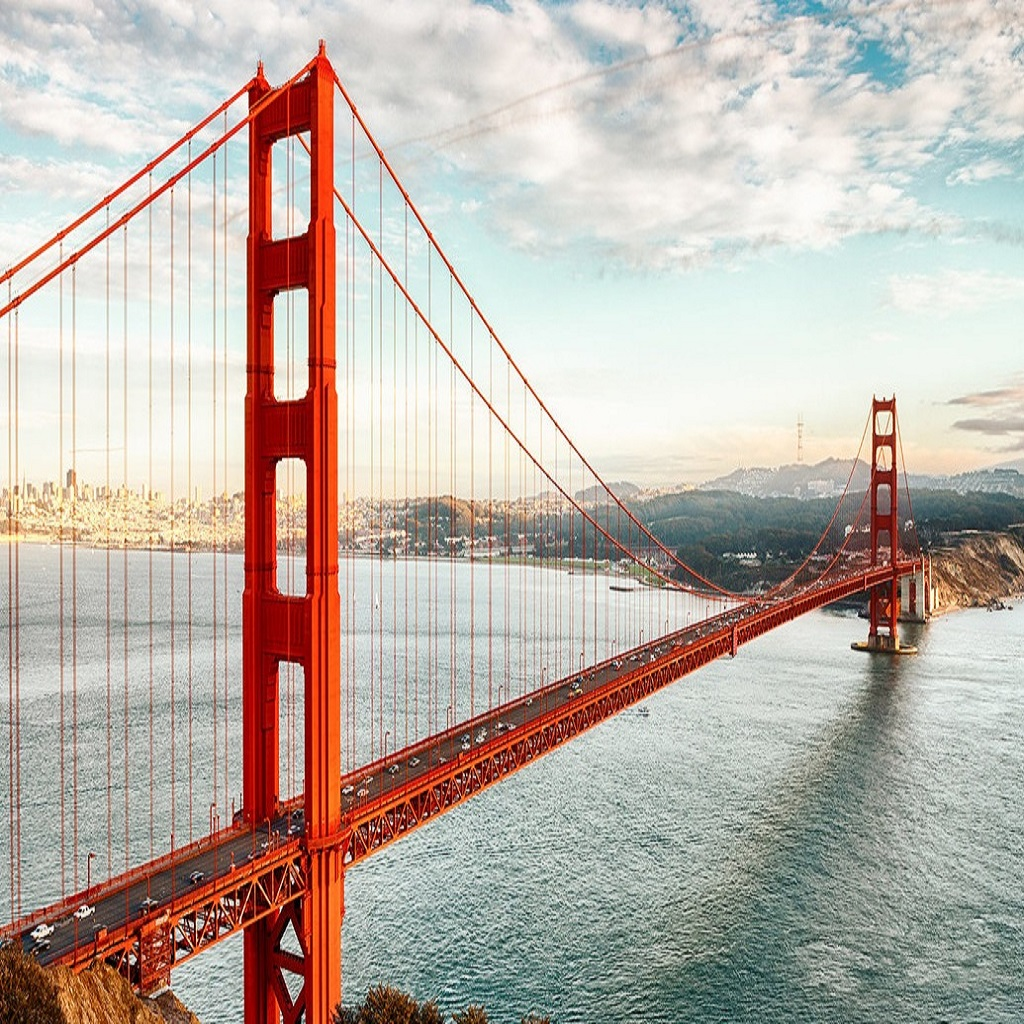
\includegraphics[width=\linewidth]{bridge_sq.jpg} % content img num.1
	\end{subfigure}
	\begin{subfigure}[b]{0.225\linewidth}
		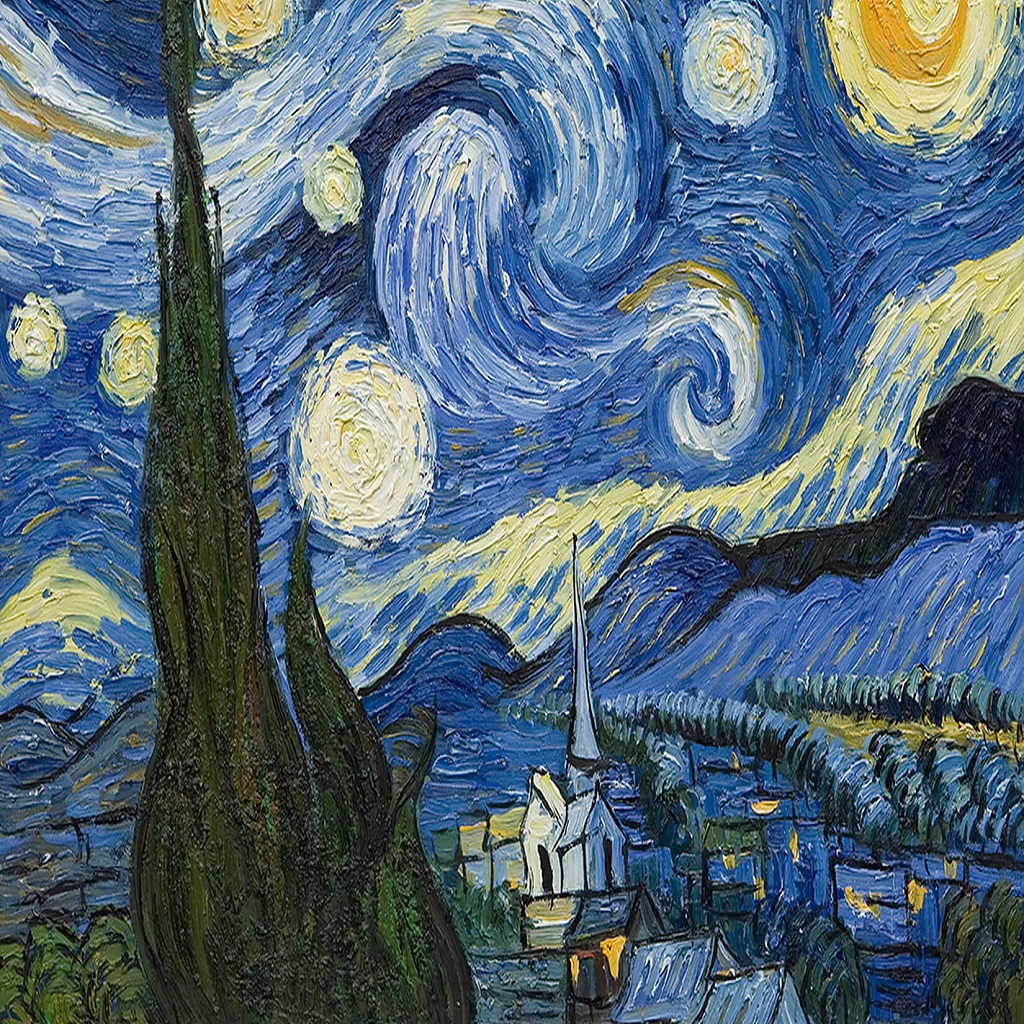
\includegraphics[width=\linewidth]{starry_sq.jpg} % style img num.1	
	\end{subfigure}
	\begin{subfigure}[b]{0.225\linewidth}
		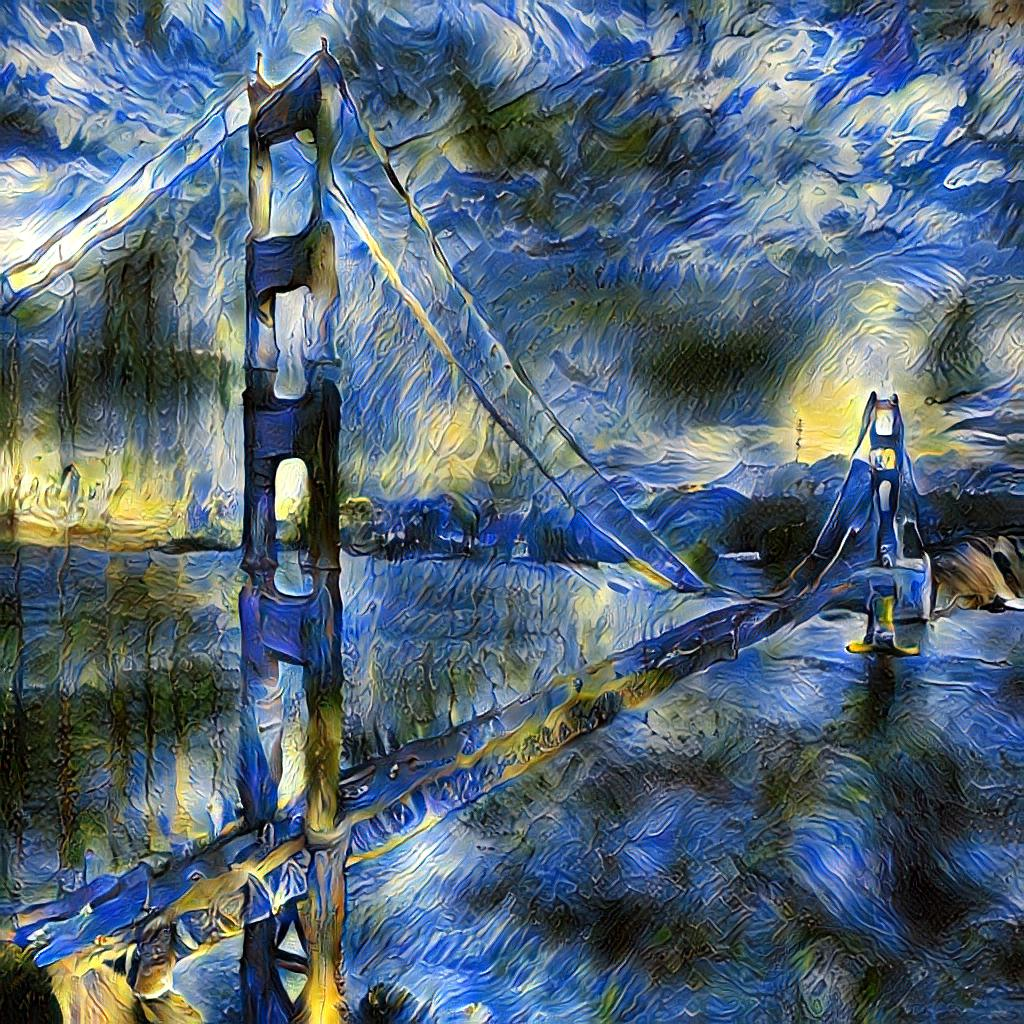
\includegraphics[width=\linewidth]{transfer_examples/transfer_bridge_starry_08_ref.jpg} % theirs reconstruction num.1	
	\end{subfigure}
	\begin{subfigure}[b]{0.225\linewidth}
		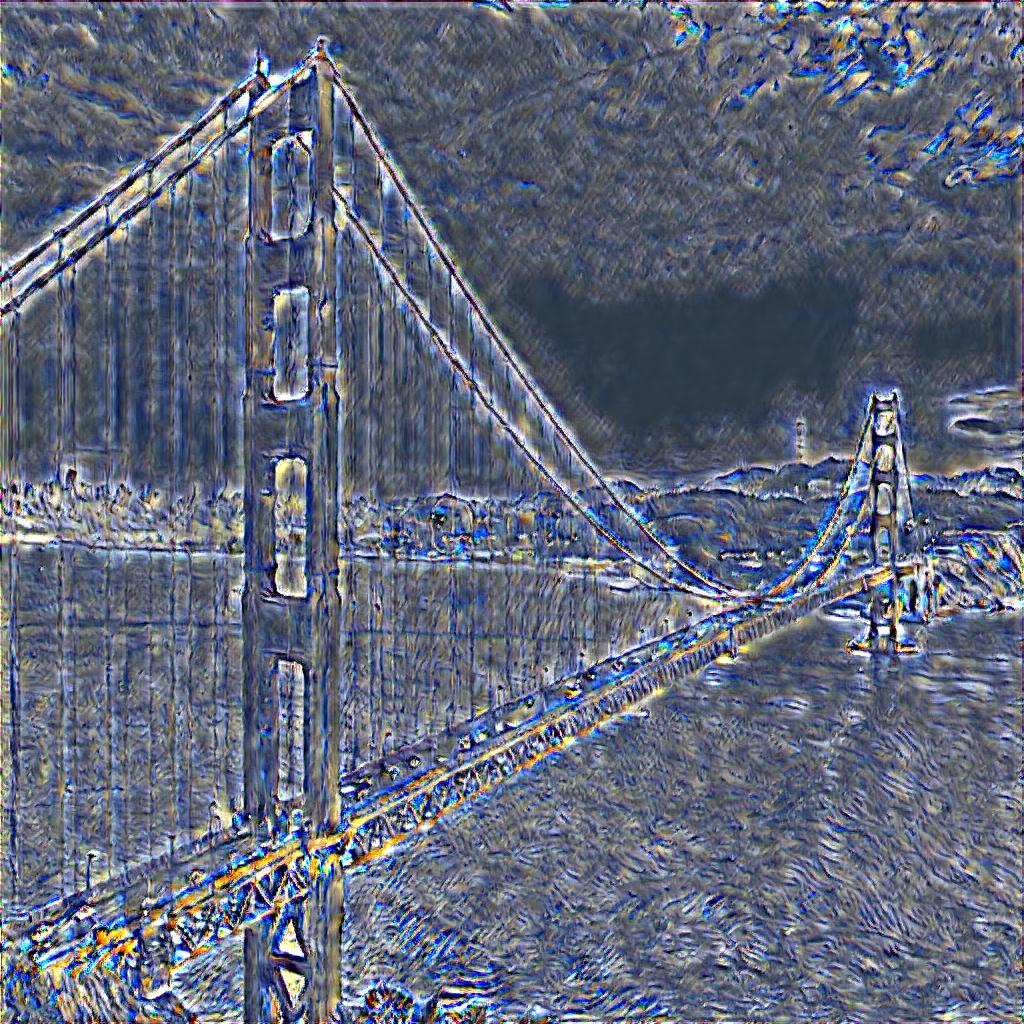
\includegraphics[width=\linewidth]{transfer_examples/transfer_bridge_starry_08_our.jpg} % ours reconstruction num.1	
	\end{subfigure}
	% second line
	\centering
	\begin{subfigure}[b]{0.225\linewidth}
		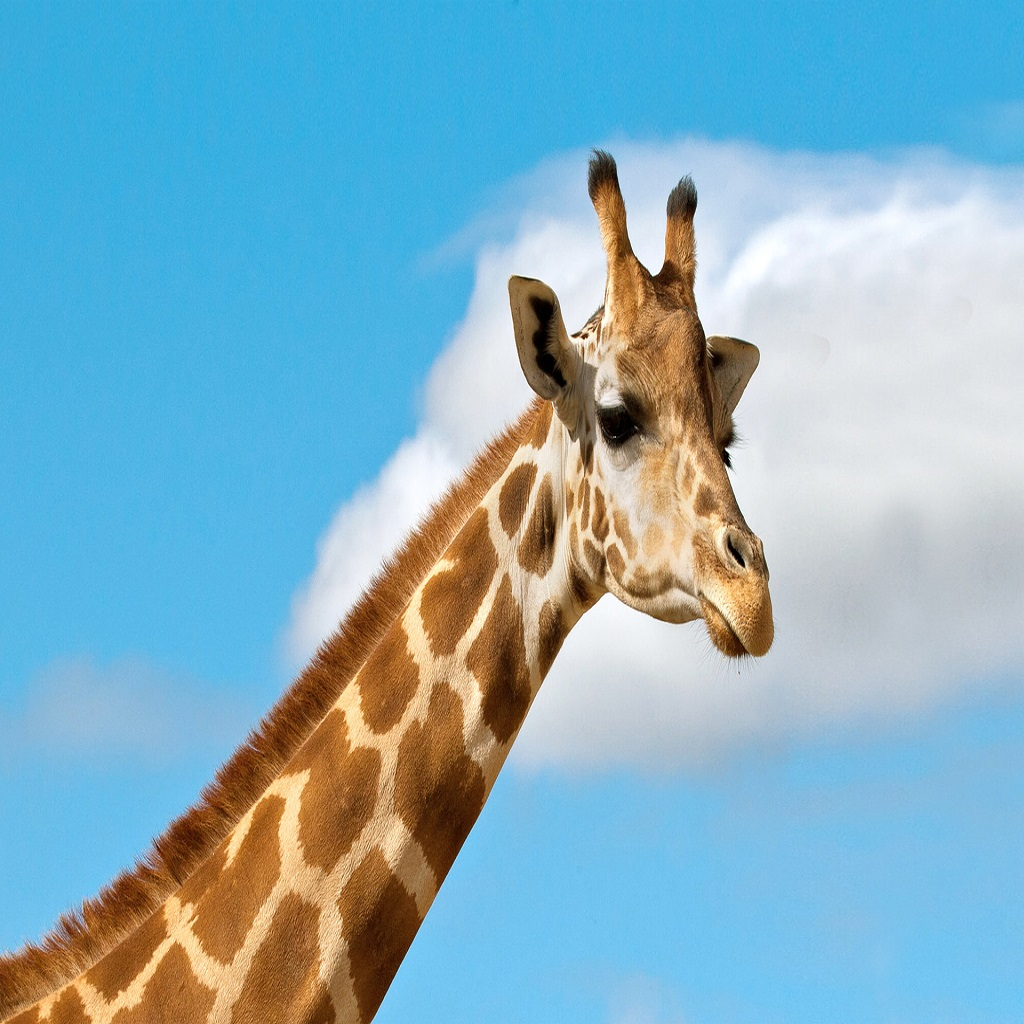
\includegraphics[width=\linewidth]{giraffe_sq.jpg} % content img num.2
	\end{subfigure}
	\begin{subfigure}[b]{0.225\linewidth}
		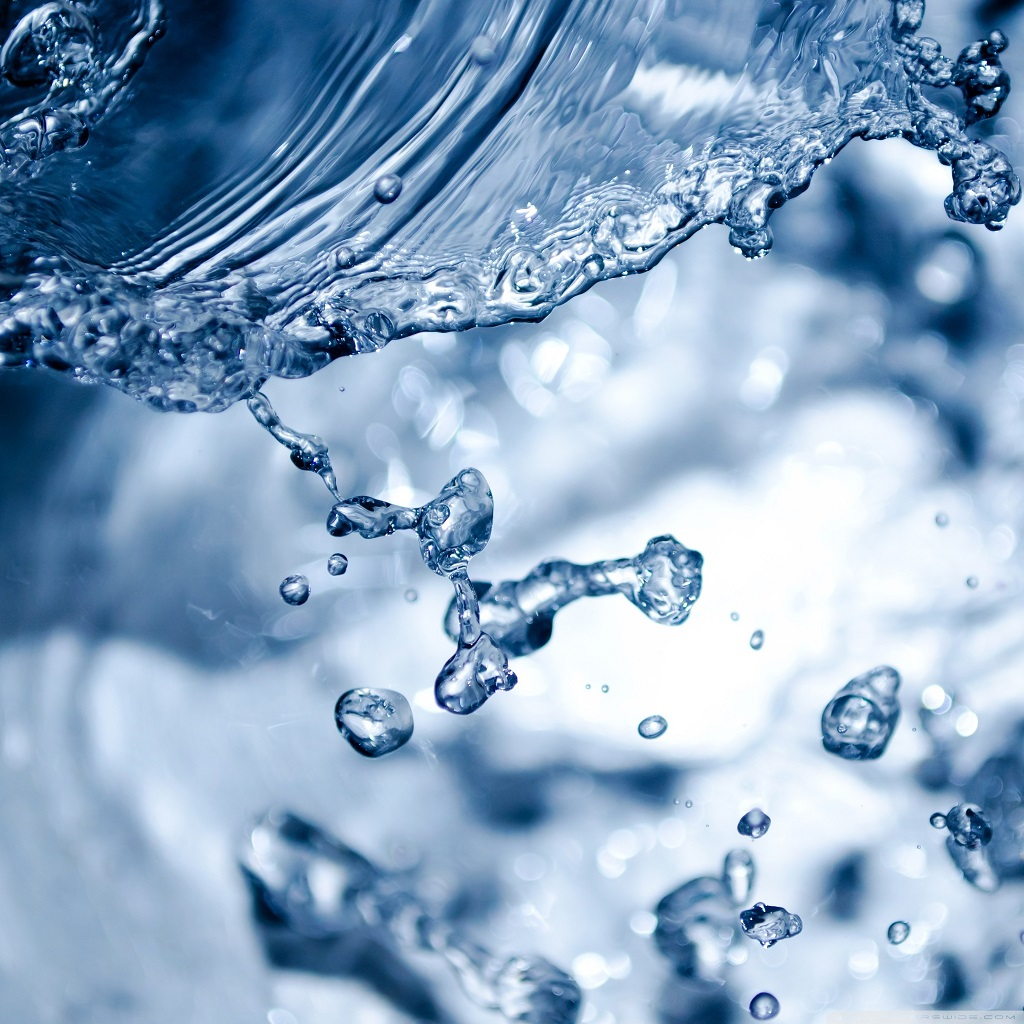
\includegraphics[width=\linewidth]{st1_sq.jpg} % style img num.2
	\end{subfigure}
	\begin{subfigure}[b]{0.225\linewidth}
		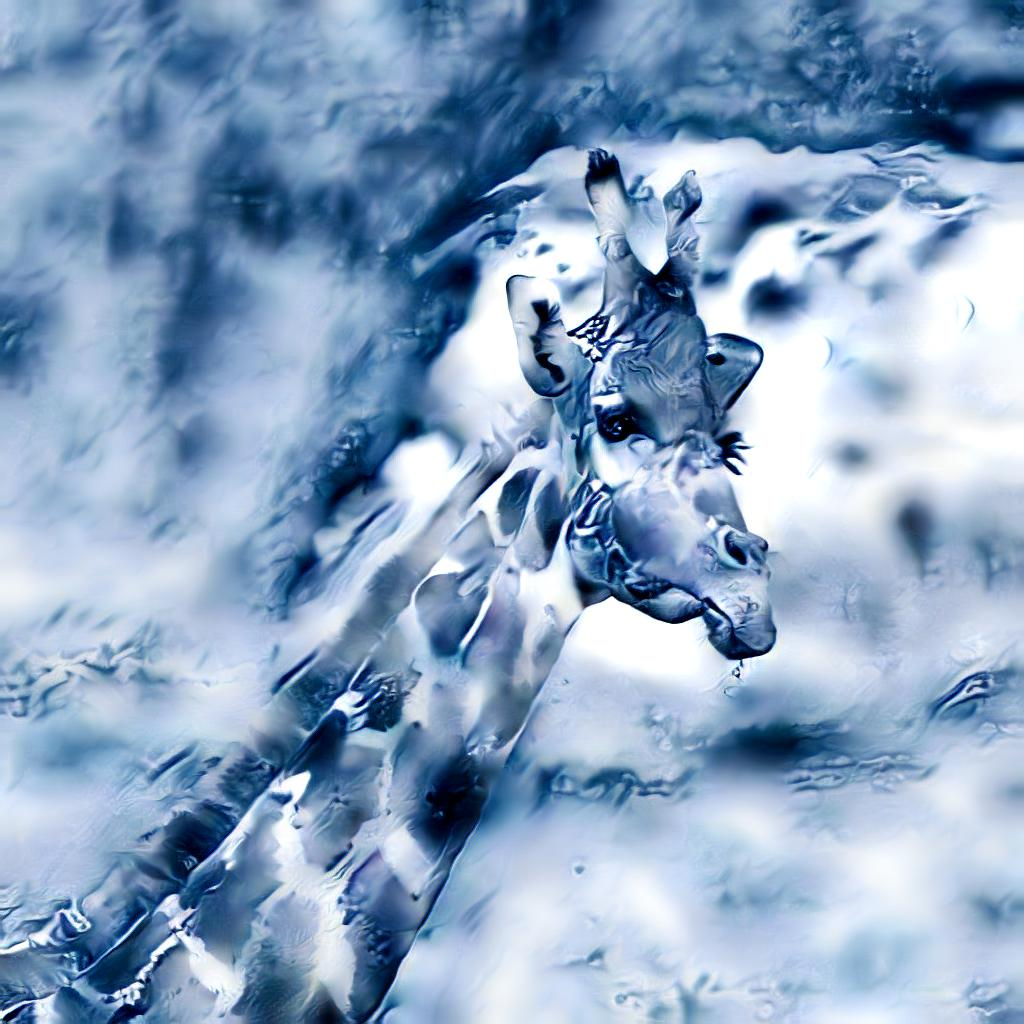
\includegraphics[width=\linewidth]{transfer_examples/transfer_giraffe_st1_08_ref.jpg} % theirs reconstruction num.2
	\end{subfigure}
	\begin{subfigure}[b]{0.225\linewidth}
		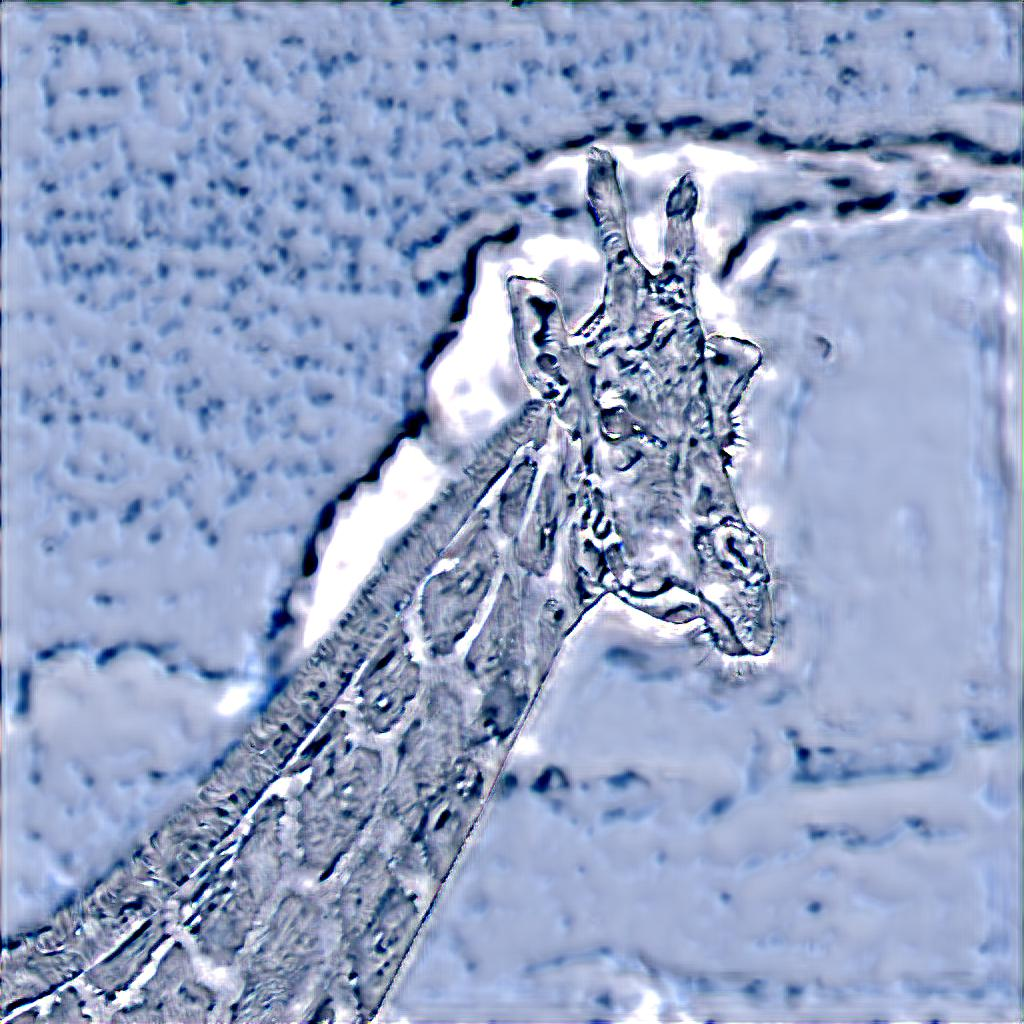
\includegraphics[width=\linewidth]{transfer_examples/transfer_giraffe_st1_08_our.jpg} % ours reconstruction num.2
	\end{subfigure}
	% third line
	\centering
	\begin{subfigure}[b]{0.225\linewidth}
		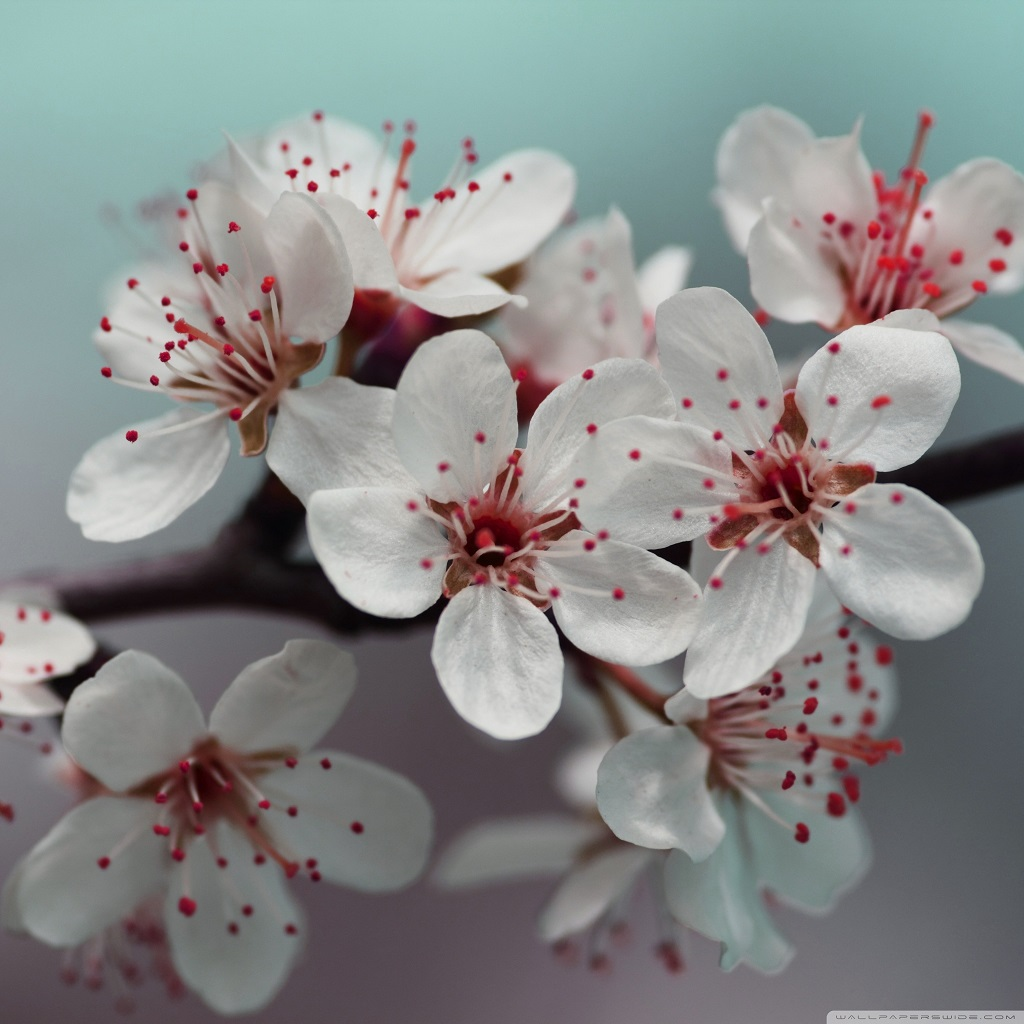
\includegraphics[width=\linewidth]{in1_sq.jpg} % content img num.3
	\end{subfigure}
	\begin{subfigure}[b]{0.225\linewidth}
		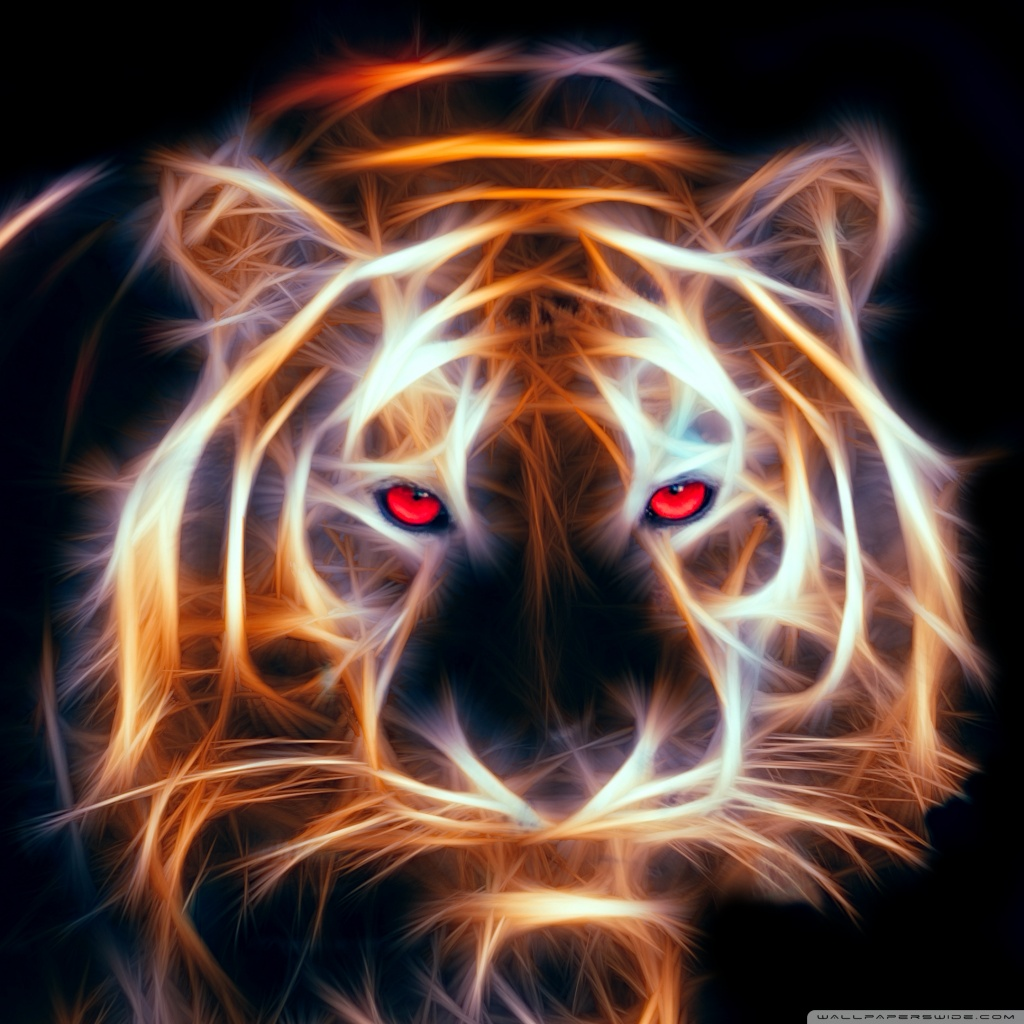
\includegraphics[width=\linewidth]{tiger_sq.jpg} % style img num.3
	\end{subfigure}
	\begin{subfigure}[b]{0.225\linewidth}
		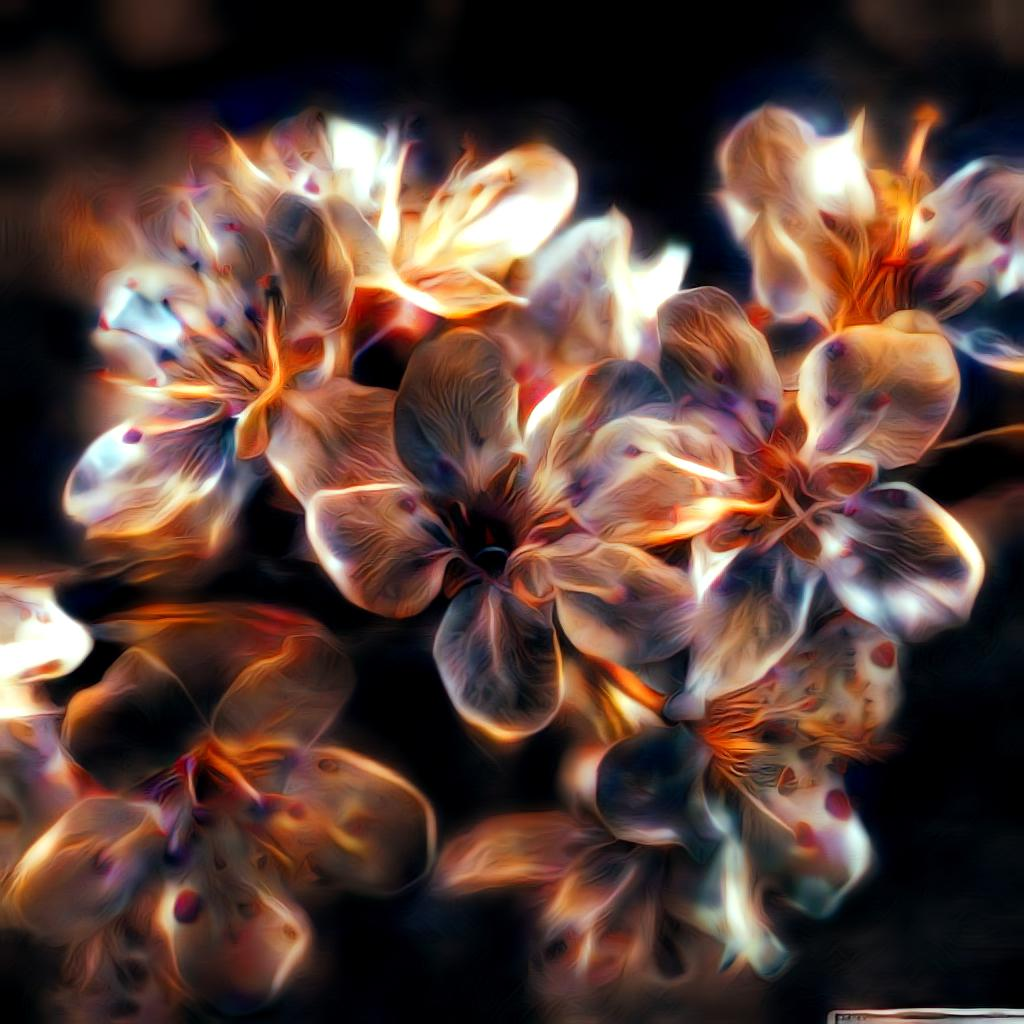
\includegraphics[width=\linewidth]{transfer_examples/transfer_in1_tiger_08_ref.jpg} % theirs reconstruction num.3
	\end{subfigure}
	\begin{subfigure}[b]{0.225\linewidth}
		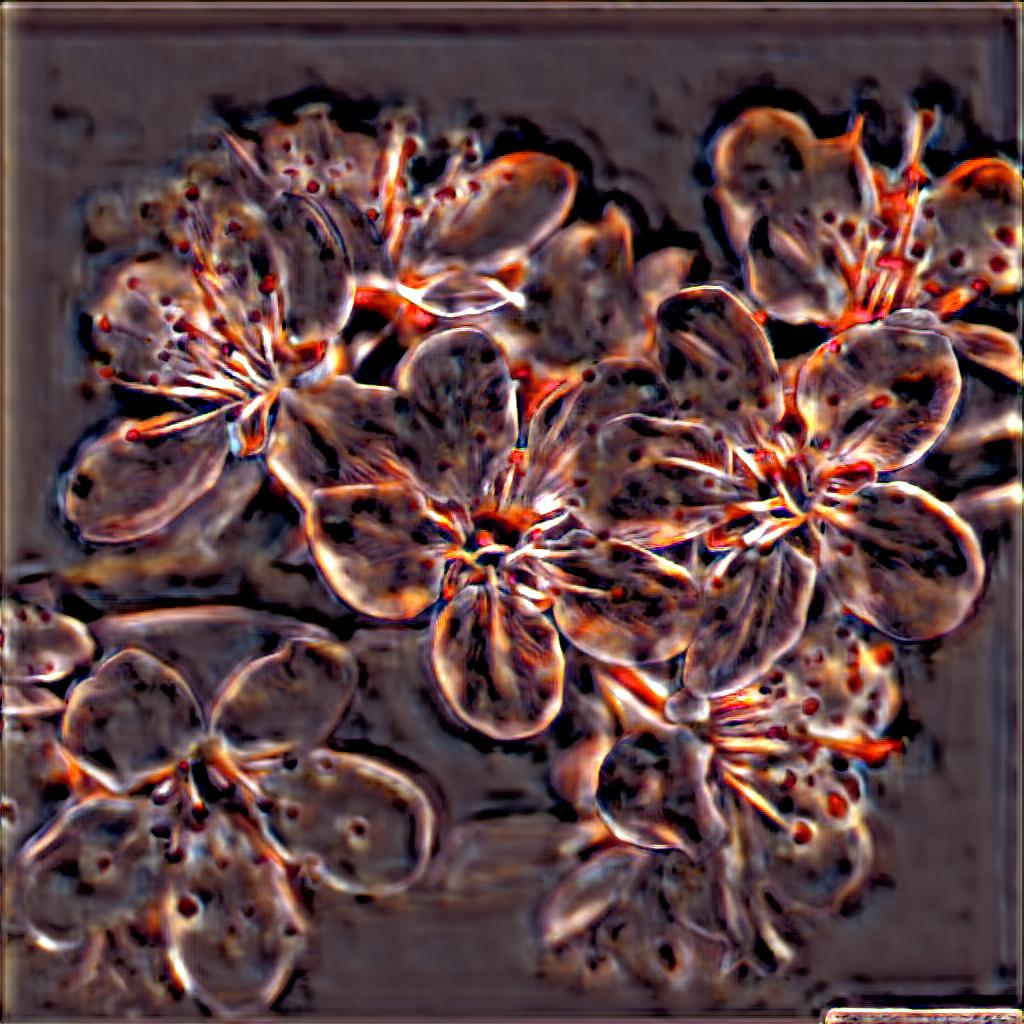
\includegraphics[width=\linewidth]{transfer_examples/transfer_in1_tiger_08_our.jpg} % ours reconstruction num.3
	\end{subfigure}
	% fourth line
	\centering
	\begin{subfigure}[b]{0.225\linewidth}
		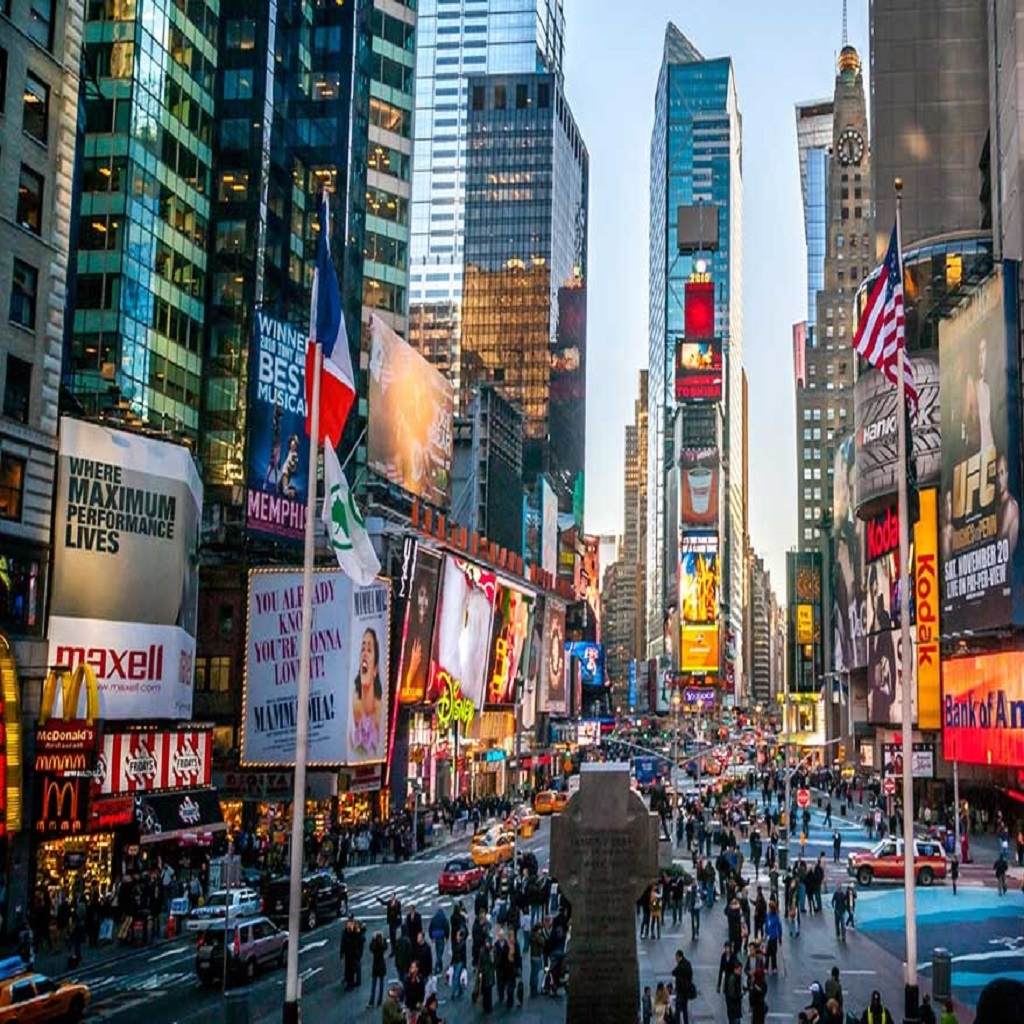
\includegraphics[width=\linewidth]{nyc_sq.jpg} % content img num.4
	\end{subfigure}
	\begin{subfigure}[b]{0.225\linewidth}
		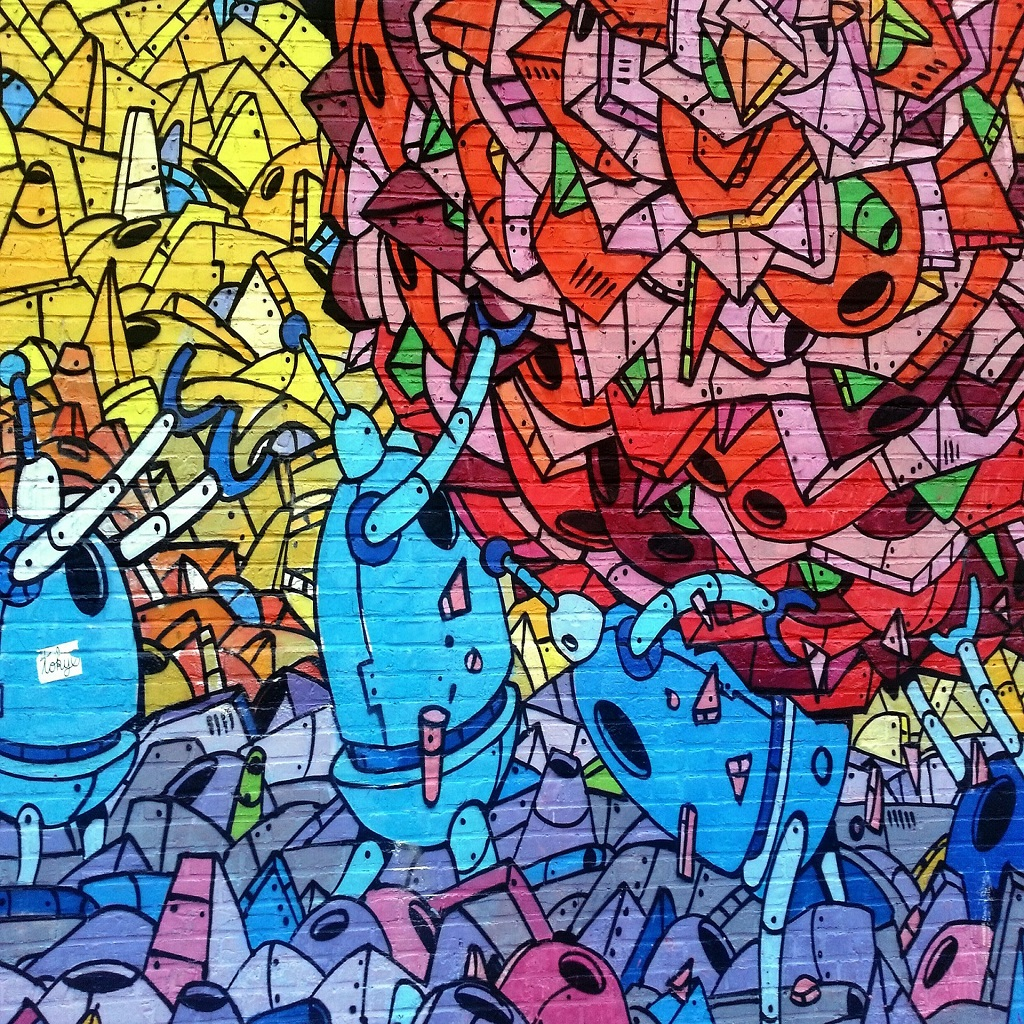
\includegraphics[width=\linewidth]{graffiti_sq.jpg} % style img num.4
	\end{subfigure}
	\begin{subfigure}[b]{0.225\linewidth}
		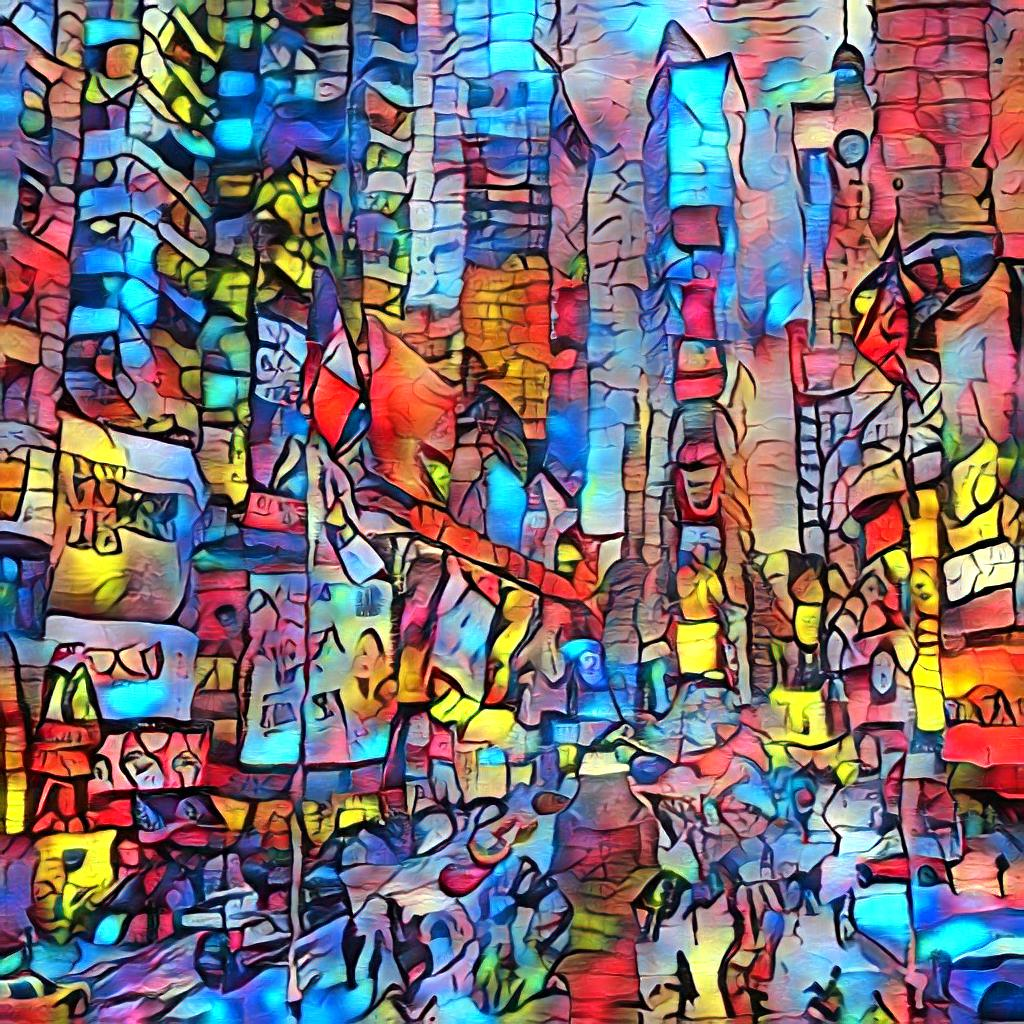
\includegraphics[width=\linewidth]{transfer_examples/transfer_nyc_graffiti_08_ref.jpg} % theirs reconstruction num.4
	\end{subfigure}
	\begin{subfigure}[b]{0.225\linewidth}
		\includegraphics[width=\linewidth]{transfer_examples/transfer_nyc_graffiti_08_our.jpg} % ours reconstruction num.4
	\end{subfigure}
	% fifth line
	\centering
	\begin{subfigure}[b]{0.225\linewidth}
		\includegraphics[width=\linewidth]{room_sq.jpg} % content img num.5
		\caption{Content}
	\end{subfigure}
	\begin{subfigure}[b]{0.225\linewidth}
		\includegraphics[width=\linewidth]{st2_sq.jpg} % style img num.5
		\caption{Style}
	\end{subfigure}
	\begin{subfigure}[b]{0.225\linewidth}
		\includegraphics[width=\linewidth]{transfer_examples/transfer_room_paint_08_ref.jpg} % theirs reconstruction num.5
		\caption{Reference Models}
	\end{subfigure}
	\begin{subfigure}[b]{0.225\linewidth}
		\includegraphics[width=\linewidth]{transfer_examples/transfer_room_paint_08_our.jpg} % ours reconstruction num.5
		\caption{Our Models}
	\end{subfigure}
	\caption{Results from different style transfer methods using style weight $\alpha=0.5$}
	\label{fig:style_transfer}
\end{figure}

It is seen in the results displayed in Figure ~\ref{fig:style_transfer} (c)+(d) that our implementation of the UST algorithm works and that given a pair of content and style images it outputs a new image that resembles the former in its content and the latter in its artistic style. As earlier mentioned the results produced by our models suffer from artifacts of gray areas originating in the reconstruction distortion. Generally column (d) shows results less pleasing than those in column (c) but clearly answers the definition of Style Transfer. \\

%%%%%%%%%%%%%%%%%%%%%%%%%%%%
%%%%%%%%%%%%%%%%%%%%%%%%%%%%
% Boost %
%%%%%%%%%%%%%%%%%%%%%%%%%%%%
%%%%%%%%%%%%%%%%%%%%%%%%%%%%
\subsubsection{Stylization boosting}
\begin{figure}[H]
	% first line
	\centering
	\begin{subfigure}[b]{0.4\linewidth}
		\includegraphics[width=\linewidth]{car_sq.jpg} % content img num.1
		%\caption{Content}
	\end{subfigure}
	\begin{subfigure}[b]{0.4\linewidth}
		\includegraphics[width=\linewidth]{st2_sq.jpg} % style img num.1
		%\caption{Style}
	\end{subfigure}
	%second line
	\begin{subfigure}[b]{0.4\linewidth}
		\includegraphics[width=\linewidth]{boost/boost_in2_st2_05_no.jpg} % regular UST num.1
		%\caption{Regular UST}
	\end{subfigure}
	\begin{subfigure}[b]{0.4\linewidth}
		\includegraphics[width=\linewidth]{boost/boost_in2_st2_05.jpg} % UST+boost num.1
		%\caption{Boost UST}
	\end{subfigure}
	\caption{First Boosting results comparing to original UST \cite{bib11}. Top left is the content image, top right is the style image, bottom left is the regular UST, bottom right is the UST+boost}
	\label{fig:Boost1}
\end{figure}
\begin{figure}[H]
	\centering
	\begin{subfigure}[b]{0.4\linewidth}
		\includegraphics[width=\linewidth]{room_sq.jpg} % content img num.1
		%\caption{Content}
	\end{subfigure}
	\begin{subfigure}[b]{0.4\linewidth}
		\includegraphics[width=\linewidth]{giraffe_sq.jpg} % style img num.1
		%\caption{Style}
	\end{subfigure}
	%second line
	\begin{subfigure}[b]{0.4\linewidth}
		\includegraphics[width=\linewidth]{boost/boost_room_giraffe_05_no.jpg} % regular UST num.1
		%\caption{Regular UST}
	\end{subfigure}
	\begin{subfigure}[b]{0.4\linewidth}
		\includegraphics[width=\linewidth]{boost/boost_room_giraffe_05.jpg} % UST+boost num.1
		%\caption{Boost UST}
	\end{subfigure}
	\caption{Second Boosting results comparing to original UST \cite{bib11}. Top left is the content image, top right is the style image, bottom left is the regular UST, bottom right is the UST+boost}
	\label{fig:Boost2}
\end{figure}
%%%%%%%%%%%%%%%%%%%%%%%% Merge  %%%%%%%%%%%%%%%%%%%%%%
\subsubsection{Two styles merging methods}
\begin{figure}[H]
	% first line
	\centering
	\begin{subfigure}[b]{0.13\linewidth}
		\includegraphics[width=\linewidth]{bridge_sq.jpg} % content img num.1
	\end{subfigure}
	\begin{subfigure}[b]{0.13\linewidth}
		\includegraphics[width=\linewidth]{starry_sq.jpg} % style1 img num.1
	\end{subfigure}
	\begin{subfigure}[b]{0.13\linewidth}
		\includegraphics[width=\linewidth]{st2_sq.jpg} % style2 img num.1
	\end{subfigure}
	\begin{subfigure}[b]{0.13\linewidth}
		\includegraphics[width=\linewidth]{merge/merge_bridge_starry_st2_1.jpg} % orig merge num.1
	\end{subfigure}
	\begin{subfigure}[b]{0.13\linewidth}
		\includegraphics[width=\linewidth]{merge/merge_bridge_starry_st2_4.jpg} % merge1 num.1
	\end{subfigure}
	\begin{subfigure}[b]{0.13\linewidth}
		\includegraphics[width=\linewidth]{merge/merge_bridge_starry_st2_2.jpg} % merge2 num.1
	\end{subfigure}
	\begin{subfigure}[b]{0.13\linewidth}
		\includegraphics[width=\linewidth]{merge/merge_bridge_starry_st2_3.jpg} % merge3 num.1
	\end{subfigure}
	% second line
	\centering
	\begin{subfigure}[b]{0.13\linewidth}
		\includegraphics[width=\linewidth]{face_sq.jpg} % content img num.2
	\end{subfigure}
	\begin{subfigure}[b]{0.13\linewidth}
		\includegraphics[width=\linewidth]{brick_sq.jpg} % style1 img num.2
	\end{subfigure}
	\begin{subfigure}[b]{0.13\linewidth}
		\includegraphics[width=\linewidth]{graffiti_sq.jpg} % style2 img num.2
	\end{subfigure}
	\begin{subfigure}[b]{0.13\linewidth}
		\includegraphics[width=\linewidth]{merge/merge_face_brick_graffiti_1.jpg} % orig merge num.2
	\end{subfigure}
	\begin{subfigure}[b]{0.13\linewidth}
		\includegraphics[width=\linewidth]{merge/merge_face_brick_graffiti_4.jpg} % merge1 num.2
	\end{subfigure}
	\begin{subfigure}[b]{0.13\linewidth}
		\includegraphics[width=\linewidth]{merge/merge_face_brick_graffiti_2.jpg} % merge2 num.2
	\end{subfigure}
	\begin{subfigure}[b]{0.13\linewidth}
		\includegraphics[width=\linewidth]{merge/merge_face_brick_graffiti_3.jpg} % merge3 num.2
	\end{subfigure}
	% third line
	\centering
	\begin{subfigure}[b]{0.13\linewidth}
		\includegraphics[width=\linewidth]{in1_sq.jpg} % content img num.3
		\caption{Content \\ image}
	\end{subfigure}
	\begin{subfigure}[b]{0.13\linewidth}
		\includegraphics[width=\linewidth]{st1_sq.jpg} % style1 img num.3
		\caption{$1^{st}$ \\ Style}
	\end{subfigure}
	\begin{subfigure}[b]{0.13\linewidth}
		\includegraphics[width=\linewidth]{tiger_sq.jpg} % style2 img num.3
		\caption{$2^{nd}$ \\ Style}
	\end{subfigure}
	\begin{subfigure}[b]{0.13\linewidth}
		\includegraphics[width=\linewidth]{merge/merge_in1_st1_tiger_1.jpg} % orig merge num.3
		\caption{Original Merge}
	\end{subfigure}
	\begin{subfigure}[b]{0.13\linewidth}
		\includegraphics[width=\linewidth]{merge/merge_in1_st1_tiger_4.jpg} % merge1 num.3
		\caption{Interp. Merge}
	\end{subfigure}
	\begin{subfigure}[b]{0.13\linewidth}
		\includegraphics[width=\linewidth]{merge/merge_in1_st1_tiger_2.jpg} % merge2 num.3
		\caption{Channel Merge}
	\end{subfigure}
	\begin{subfigure}[b]{0.13\linewidth}
		\includegraphics[width=\linewidth]{merge/merge_in1_st1_tiger_3.jpg} % merge3 num.3
		\caption{Level Merge}
	\end{subfigure}
		\caption{Results using different stylization methods.}
		\label{fig:Merge}
\end{figure}
%%%%%%%%%%%%%%%%%%%%%%%%%%%%
add more text here\newline
%%%%%%%%%%%%%%%%%%%%%%%%%%%%%%%
\textbf{Style-Merging Methods Efficiency}
%Efficiency table%
\begin{center}
	\captionof{table}{UST merge runtime of different techniques\label{Tab:merge}}
	\begin{tabular}{||c| |c| |c| |c| |c||} 
		\hline
		\space & Original & Interpolation & Channel & Level \\ [0.5ex] 
		\hline\hline
		Time[sec] & 7.42 & 6.94 & 6.80 & 6.17\\ 
		\hline
	\end{tabular}
\end{center}

%%%%%%%%%%%%%%%%%%%%%%%% Texture synthesis  %%%%%%%%%%%%%%%%%%%%%%
\subsubsection{Texture synthesis}
We demonstrate the effectiveness of our method for universal style transfer by showing its application to universal texture synthesis. In figure ~\ref{fig:texture} we visualize the whitened features and
synthesized textures via simple feature coloring.
One option to produce texture image is simply setting the content image as a random noise image (e.g., Gaussian noise). Another option to get synthesized texture in our stylization framework is to directly initialize the content features to be white noise as proposed by Li et al. \cite{bib11}. Both approaches achieve similar results.
The evaluation criterion for the quality of the synthesized texture is usually human inspection and textures are successfully synthesized if a human observer cannot tell the original texture from a synthesized one.
\begin{figure}[H]
	% first line
	\centering
	\begin{subfigure}[b]{0.4\linewidth}
		\includegraphics[width=\linewidth]{brick_sq.jpg} %style img num.1
	\end{subfigure}
	\begin{subfigure}[b]{0.4\linewidth}
		\includegraphics[width=\linewidth]{texture_synth/brick_tex.jpg} % stylization img num.1
	\end{subfigure}
	% second line
	\centering
	\begin{subfigure}[b]{0.4\linewidth}
		\includegraphics[width=\linewidth]{cubism2_sq.jpg} %style img num.2
		\caption{Style}
	\end{subfigure}
	\begin{subfigure}[b]{0.4\linewidth}
		\includegraphics[width=\linewidth]{texture_synth/cubism2_tex.jpg} % stylization img num.2
		\caption{Our UST}
	\end{subfigure}
	\caption{Synthesized results.}
	\label{fig:texture}
\end{figure}